\documentclass[conference]{IEEEtran}
\IEEEoverridecommandlockouts
\usepackage{mathptmx} % Times for text and math: one font family throughout
\usepackage{cite}
\usepackage{amsmath,amssymb,amsfonts}
\usepackage{algorithm}
\usepackage{algpseudocode}
\makeatletter
% section titles and table captions in italic instead of small caps
\def\section{\@startsection{section}{1}{\z@}{1.5ex plus 1.5ex minus 0.5ex}{0.7ex plus 1ex minus 0ex}{\normalfont\normalsize\centering\itshape}}
\long\def\@makecaption#1#2{%
\ifx\@captype\@IEEEtablestring
\footnotesize\bgroup\par\centering\@IEEEtabletopskipstrut{\normalfont\footnotesize #1}\\{\normalfont\footnotesize\itshape #2}\par\addvspace{0.5\baselineskip}\egroup
\@IEEEtablecaptionsepspace
\else
\@IEEEfigurecaptionsepspace
\setbox\@tempboxa\hbox{\normalfont\footnotesize {#1.}\nobreakspace\nobreakspace #2}%
\ifdim \wd\@tempboxa >\hsize
\setbox\@tempboxa\hbox{\normalfont\footnotesize {#1.}\nobreakspace\nobreakspace}%
\parbox[t]{\hsize}{\normalfont\footnotesize\noindent\unhbox\@tempboxa#2}%
\else
\hbox to\hsize{\normalfont\footnotesize\hfil\box\@tempboxa\hfil}%
\fi\fi}
\let\oldfsruled\fs@ruled
\renewcommand\fs@ruled{\oldfsruled\def\@fs@cfont{\normalfont}}
\makeatother
\restylefloat{algorithm}
\usepackage{graphicx}
\usepackage{booktabs}
\usepackage{multirow}
\usepackage{xcolor}
\usepackage{tikz}
\usepackage{pgfplots}
\pgfplotsset{compat=1.16}
\usetikzlibrary{calc}
\usetikzlibrary{positioning,arrows.meta,fit}
\usepackage[hidelinks]{hyperref}
\usepackage{balance}
\usepackage{amsthm}
\newtheoremstyle{plainhead}{3pt}{3pt}{\itshape}{}{\normalfont}{.}{.5em}{}
\theoremstyle{plainhead}
\newtheorem{proposition}{Proposition}
\algrenewcommand\algorithmicrequire{Require:}
\algrenewcommand\algorithmicfor{for}
\algrenewcommand\algorithmicdo{do}
\algrenewcommand\algorithmicend{end}
\algrenewcommand\algorithmicreturn{return}
\algrenewcommand\algorithmicwhile{while}
\algrenewcommand\algorithmicif{if}
\algrenewcommand\algorithmicthen{then}

\newcommand{\iws}{\textit{IWS}}
\usepackage{xspace}
\newcommand{\pp}{\,pp\xspace}

\begin{document}

\title{When Does a Machine Learning Model Fail?\\
Linking Feature-Space Changes to Prediction Degradation}

% ---- Replace with your details (remove for double-blind review) ----
\author{\IEEEauthorblockN{First Author}
\IEEEauthorblockA{\textit{Department} \\
\textit{Institution}\\
City, Country \\
email@domain}
\and
\IEEEauthorblockN{Second Author}
\IEEEauthorblockA{\textit{Department} \\
\textit{Institution}\\
City, Country \\
email@domain}}

\maketitle

\begin{abstract}
Deployed models are routinely monitored with drift detectors that raise an alarm whenever the input distribution changes, yet a change in $P(X)$ need not change the error of the model. This research asks which measurable feature-space changes actually predict prediction degradation, and why the rest do not. The proposed methodology assembles a testbed of 173 natural source$\to$target shifts drawn from seven public tabular datasets (demographic, geographic, temporal and carrier splits), trains three model classes with three seeds each (1{,}557 evaluations), and compares thirteen label-free signals against the true accuracy drop. The proposed methodology also introduces \emph{Importance-Weighted Shift} (\iws{}), which weights each feature's drift by the model's own reliance on that feature, and a reweighting decomposition that separates the covariate part of a drop from the conditional part. Three findings stand out. First, drift is nearly universal but weakly informative: a domain classifier separates source from target with AUC $\ge 0.95$ in 68\% of pairs, while 25\% of drifted evaluations show no harm and 48\% of low-drift evaluations still fail. Second, \iws{} gives the best harm detection among single signals (AUROC 0.70, AUPRC 0.86) and the highest rank correlation with the drop ($\rho=0.42$), whereas confidence-based estimators that work well on images correlate weakly on tabular shifts ($\rho \approx 0.07$). Third, in 76\% of harmful evaluations the conditional part $P(Y|X)$ dominates the covariate part, and controlled experiments confirm that such concept shift is invisible to every label-free signal. Code and results are released to support reproducible monitoring research.
\end{abstract}

\par\vspace{4pt}\noindent{\normalfont\small\textit{Index Terms}---
distribution shift, concept drift, model monitoring, performance estimation, tabular data, feature importance}\par

% =====================================================================
\section{Introduction}
% =====================================================================
A model that was accurate at validation time can quietly lose accuracy after deployment because the data it receives no longer resembles the data it was trained on~\cite{hinder2024a,liu2023need}. Labels that would reveal the loss usually arrive late or never, so practitioners rely on \emph{drift detectors}: univariate tests such as Kolmogorov--Smirnov (KS) or the Population Stability Index (PSI), kernel two-sample tests~\cite{biggs2023mmdfuse}, or classifier two-sample tests~\cite{pandeva2024e,nguyen2025reliably}. These tools answer the question ``has $P(X)$ changed?''. The question an operator actually needs answered is different: ``will my model now make more mistakes?''.

The two questions come apart for two reasons. A change confined to features the model ignores is harmless, yet it triggers every detector. Conversely, a change in the relation between features and label, $P(Y|X)$, can destroy accuracy while leaving $P(X)$ untouched, so no detector fires. Recent work on tabular benchmarks found that such conditional shifts are common in practice~\cite{liu2023need}, and that the accuracy gap tracks label-distribution shift~\cite{gardner2023tableshift}. What is missing is a direct, large-scale measurement of how well each label-free signal predicts the actual drop, and of \emph{why} it fails when it does.

This research provides that measurement and makes four contributions. The first is a \textit{shift--degradation testbed}: 173 natural source$\to$target pairs from seven public tabular datasets, three model classes and three seeds, giving 1{,}557 evaluations, each with its true accuracy drop and 13 label-free signals. The second is \textit{Importance-Weighted Shift} (\iws{}), a simple model-aware statistic that weights per-feature drift by permutation importance; it is the best single predictor of harm in the proposed testbed and costs one importance computation per deployed model. The third is a \textit{covariate/conditional decomposition} of each drop by density-ratio reweighting, validated on synthetic shifts with known ground truth, which shows that conditional shift dominates natural tabular failures. The fourth is a \textit{failure taxonomy} (stable, benign drift, harmful covariate shift, conditional failure) with practical guidance on when a drift alarm should trigger retraining.

% =====================================================================
\section{Related Work}
% =====================================================================
\textit{Shift detection.} Concept-drift research monitors streams for changes and has been surveyed for both detection and explanation~\cite{hinder2024a,hinder2024b}. For batch shift, kernel tests~\cite{biggs2023mmdfuse} and deep classifier two-sample tests~\cite{pandeva2024e} are effective at \emph{detecting} shift. Detection, however, is not harm: these tests report shift presence, not its effect on error.

\textit{Label-free performance estimation.} Several methods predict target accuracy from unlabeled data: confidence-based estimators such as Average Thresholded Confidence (ATC) and difference of confidences (DoC), evaluated and extended by prediction-matrix~\cite{deng2023confidence} and matrix-norm~\cite{xie2024mano} scores; importance-weighted estimators under covariate shift~\cite{kato2023double}; and calibrated density-ratio estimation in PAPE~\cite{bialek2025pape}. Most were validated on image benchmarks; their behaviour on natural tabular shifts with strong conditional components is less understood.

\textit{Harmful-shift testing.} Detectron~\cite{ginsberg2023detectron}, Amoukou~\textit{et~al.}~\cite{amoukou2024sequential} and Nguyen~\textit{et~al.}~\cite{nguyen2025reliably} detect harmful shift without labels. These methods output an alarm, not an explanation of which features or which kind of shift caused it.

\textit{Tabular shift benchmarks.} TableShift~\cite{gardner2023tableshift} and the WhyShift study~\cite{liu2023need} collect natural shifts on tabular data and show that the accuracy gap depends on which part of the joint distribution moves, while a large comparison of boosted trees and neural networks~\cite{mcelfresh2023neural} shows that no model family wins on every dataset. These resources measure how large the accuracy gap is; the proposed methodology measures how well label-free signals predict it, which is the question a deployed monitor has to answer.

\textit{Explaining shifts and drops.} Zhang~\textit{et~al.}~\cite{zhang2023why} attribute a drop to shifted causal mechanisms with Shapley values; DISDE~\cite{cai2023diagnosing} splits a drop into harder examples, conditional shift and unseen examples; Kulinski and Inouye~\cite{kulinski2023explaining} explain shifts via transport maps. Explanation shift~\cite{mougan2023explanation} monitors SHAP distributions, Decker~\textit{et~al.}~\cite{decker2024explanatory} explain the effect of feature shifts on performance, while FMMO~\cite{zafar2026fmmo} shows local attributions can stay stable as error rises. The proposed methodology is complementary: rather than proposing one more detector, the research work measures which signals track degradation across many natural shifts and explains the misses with a decomposition.

% =====================================================================
\section{Problem Formulation}
% =====================================================================
Let $P_S(X,Y)$ be the source distribution on which a classifier $f$ is trained, and $P_T(X,Y)$ a deployment distribution. Labelled source validation data $\{(x_i,y_i)\}_{i=1}^{n_S}$ and \emph{unlabelled} target features $\{x_j\}_{j=1}^{n_T}$ are available. The \textit{accuracy drop} is
\begin{equation}
\Delta = \mathrm{Acc}_S(f) - \mathrm{Acc}_T(f),
\end{equation}
and a shift is \textit{harmful} if $\Delta>\tau$ (default $\tau = 2$\pp; Sec.~\ref{sec:ablation} varies $\tau$). Writing $P(X,Y)=P(X)P(Y|X)$, a \emph{covariate} shift changes only $P(X)$, a \emph{conditional} (concept) shift changes $P(Y|X)$, and a \emph{label} shift changes $P(Y)$ with $P(X|Y)$ fixed~\cite{liu2023need,kimura2025graph}. A \textit{signal} is any statistic $s(f,\mathcal{D}_S,\{x_j\})$ computed without target labels. The goal of the proposed methodology is to measure how well each $s$ ranks pairs by $\Delta$ and separates harmful from benign shifts.

% =====================================================================
\section{Method}
% =====================================================================
Fig.~\ref{fig:pipeline} summarizes the study: label-free signals are computed exactly as a monitor would compute them; target labels are used only afterwards, to score the signals.

\begin{figure}[t]
\centering
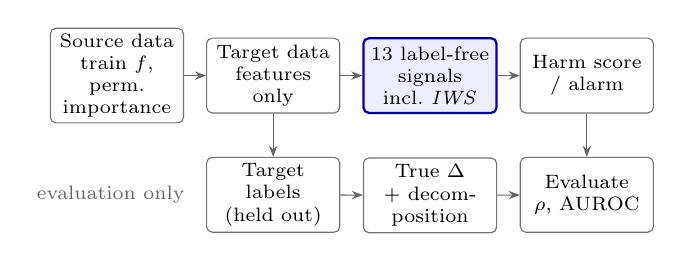
\begin{tikzpicture}[
  box/.style={draw=black!55, rounded corners=2pt, align=center, font=\scriptsize,
              minimum height=0.95cm, text width=1.55cm, inner sep=2pt},
  hl/.style={box, draw=blue!70!black, fill=blue!7, thick},
  arr/.style={-{Stealth[length=4pt]}, black!60}]
\node[box] (src) {Source data\\ train $f$, perm.\ importance};
\node[box, right=0.28cm of src] (tgt) {Target data\\ features only};
\node[hl, right=0.28cm of tgt] (sig) {13 label-free signals incl.\ \iws{}};
\node[box, right=0.28cm of sig] (harm) {Harm score / alarm};
\node[box, below=0.55cm of tgt] (lab) {Target labels\\ (held out)};
\node[box, below=0.55cm of sig] (dec) {True $\Delta$ + decomposition};
\node[box, below=0.55cm of harm] (ev) {Evaluate\\ $\rho$, AUROC};
\draw[arr] (src) -- (tgt); \draw[arr] (tgt) -- (sig); \draw[arr] (sig) -- (harm);
\draw[arr] (tgt) -- (lab); \draw[arr] (lab) -- (dec); \draw[arr] (dec) -- (ev); \draw[arr] (harm) -- (ev);
\node[font=\scriptsize, text=black!60, anchor=east] at ([xshift=-0.15cm]lab.west) {evaluation only};
\end{tikzpicture}
\caption{Study pipeline. The top row is what a deployed monitor sees; the bottom row exists only to score how well each signal predicts the real drop.}
\label{fig:pipeline}
\end{figure}

\subsection{Label-free signals}
The thirteen signals are grouped by what they look at.

\textit{Data-only (D).} Mean and maximum per-feature KS statistic; mean per-feature Wasserstein-1 distance on source-standardized features; mean PSI with ten source-quantile bins; unbiased MMD$^2$ with an RBF kernel and median-heuristic bandwidth~\cite{biggs2023mmdfuse}; and the AUC of a domain classifier (gradient-boosted trees, 3-fold cross-fitting) that separates source from target rows~\cite{pandeva2024e,nguyen2025reliably}.

\textit{Model-aware drift (M), proposed.} Let $d_j$ be the drift of feature $j$ (KS statistic or standardized Wasserstein distance) and $I_j$ the permutation importance~\cite{chamma2024variable} of feature $j$ for model $f$, measured as the accuracy loss on source validation data when feature $j$ is shuffled. With $w_j=\max(I_j,0)/\sum_k \max(I_k,0)$,
\begin{equation}
\iws(f) \;=\; \sum_{j=1}^{p} w_j\, d_j .
\label{eq:iws}
\end{equation}
\iws{} is zero when only ignored features move and large when the features the model relies on move. It needs source labels once (for $w$) and no target labels. The proposed methodology reports \iws{}-KS and \iws{}-Wass. The following observation motivates the weighting.

\begin{proposition}
Let $U\subseteq\{1,\dots,p\}$ be the features $f$ depends on, so $f(x)=g(x_U)$, and suppose $P_T(Y|X)=P_S(Y|X)$ with $P(Y|X)$ depending on $x$ only through $x_U$. If the shift leaves the marginal of $X_U$ unchanged, $P_T(x_U)=P_S(x_U)$, then $\Delta=0$, however large the drift of the features outside $U$.
\end{proposition}
\begin{proof}
$\mathrm{Acc}_D(f)=\mathbb{E}_{x_U\sim P_D}\big[P(Y{=}g(x_U)\mid x_U)\big]$ for $D\in\{S,T\}$. The integrand is the same function under $S$ and $T$, and so is the distribution it is integrated against; hence $\mathrm{Acc}_S=\mathrm{Acc}_T$.
\end{proof}

Data-only detectors respond to the drift of all $p$ features and so cannot respect this invariance; \iws{} approximates it by giving zero weight to features with zero importance. The converse does not hold: drift in $X_U$ can even raise accuracy (Sec.~\ref{sec:synth}), and a change in $P(Y|X)$ is invisible to any function of $X$ alone.

\textit{Model-output (O).} Following the confidence-based estimators evaluated in~\cite{deng2023confidence,xie2024mano}: drop in mean maximum class probability, i.e.\ difference of confidences (DoC); absolute change in predicted positive rate; ATC drop, i.e.\ source accuracy minus the ATC target estimate; importance-weighted drop (IW-drop), i.e.\ source accuracy minus the density-ratio-weighted source accuracy~\cite{kato2023double}; and the increase in disagreement between $f$ and a reference model of a different class.

\subsection{Covariate/conditional decomposition}
\label{sec:decomp}
The domain classifier gives out-of-fold probabilities $\hat p(T|x)$ for source rows, from which density-ratio weights are formed, $\hat r(x)=\frac{\hat p(T|x)}{1-\hat p(T|x)}\cdot\frac{n_S}{n_T}$ (probabilities clipped to $[0.01,0.99]$, weights capped at 50). The weighted source accuracy
\begin{equation}
\widehat{\mathrm{Acc}}_{S\to T}=\frac{\sum_i \hat r(x_i)\,\mathbb{1}[f(x_i)=y_i]}{\sum_i \hat r(x_i)}
\end{equation}
estimates what the target accuracy would be if only $P(X)$ had changed. The drop then splits as
\begin{equation}
\Delta=\underbrace{\mathrm{Acc}_S-\widehat{\mathrm{Acc}}_{S\to T}}_{\text{covariate part}}
+\underbrace{\widehat{\mathrm{Acc}}_{S\to T}-\mathrm{Acc}_T}_{\text{residual (conditional) part}} .
\label{eq:decomp}
\end{equation}
The covariate part is label-free (it equals IW-drop); the residual needs target labels and is used only for analysis. When source and target barely overlap, reweighting cannot represent target regions absent from the source, so the residual also absorbs out-of-support error, which DISDE~\cite{cai2023diagnosing} treats as a separate term. Results are therefore also reported on the subset with domain-classifier AUC $<0.95$.

\subsection{Harm score}
To test whether signals combine, a gradient-boosted regressor is fitted that maps all thirteen signals to $\Delta$. The regressor is evaluated \emph{leave-one-dataset-out}: the regressor never sees any pair from the dataset it is scored on.

\begin{algorithm}[t]
\caption{Computing \iws{} for a deployed model}
\label{alg:iws}
\begin{algorithmic}[1]
\Require model $f$, source validation $(X_S,y_S)$, target batch $X_T$
\State $a \gets \mathrm{Acc}(f, X_S, y_S)$
\For{$j=1,\dots,p$} \Comment{once per model}
  \State $I_j \gets a - \mathrm{Acc}(f, \mathrm{shuffle}_j(X_S), y_S)$
\EndFor
\State $w_j \gets \max(I_j,0)/\sum_k \max(I_k,0)$
\For{each new target batch $X_T$}
  \State $d_j \gets \mathrm{KS}(X_S[:,j], X_T[:,j])$ for all $j$
  \State \Return $\iws=\sum_j w_j d_j$
\EndFor
\end{algorithmic}
\end{algorithm}

% =====================================================================
\section{Experimental Setup}
% =====================================================================
\subsection{Datasets and natural shifts}
The research work uses seven public tabular datasets with natural domain structure (Table~\ref{tab:data}), drawn from public repositories and used in recent tabular shift benchmarks~\cite{gardner2023tableshift,liu2023need,mcelfresh2023neural}. Each split attribute defines domains; every ordered pair of domains with at least 400 rows becomes a source$\to$target pair, except temporal splits, where only past$\to$future pairs are kept. The split attribute itself is removed from the features. Bank Marketing has the known leakage variable ``duration'' removed and its calendar month removed for the time split. This yields 173 pairs.

\begin{table}[t]
\centering
\caption{Datasets and natural shift axes.}
\label{tab:data}
\footnotesize
\setlength{\tabcolsep}{3pt}
\begin{tabular}{lrrlr}
\toprule
Dataset & Rows & Feat. & Shift axes (domains) & Pairs \\
\midrule
Adult & 45{,}222 & 48 & sex, race, age, education, workclass & 34 \\
COMPAS & 6{,}172 & 13 & race, sex, age group & 14 \\
Housing & 20{,}428 & 15 & ocean proximity, north/south & 14 \\
Bank & 41{,}188 & 62 & time (6 blocks, 2008--10) & 15 \\
Elec2 & 45{,}312 & 6 & time (8 blocks) & 28 \\
Airlines & 381{,}161 & 5 & carrier (top 8) & 56 \\
Covertype & 581{,}012 & 54 & wilderness area (4) & 12 \\
\bottomrule
\end{tabular}
\end{table}

\subsection{Models and protocol}
The models are logistic regression, a histogram gradient-boosted tree ensemble (GBDT, a strong model family on tabular data~\cite{mcelfresh2023neural}) and a two-layer MLP (128--64 units), all trained with scikit-learn. Per source domain, up to 5{,}000 rows are held out for validation and up to 20{,}000 used for training; up to 5{,}000 target rows are sampled. Every pair is run with three seeds that change the sampling and model initialization, giving $173\times3\times3 = 1{,}557$ evaluations.

\subsection{Implementation details}
Logistic regression standardizes the features and uses an $\ell_2$ penalty with $C=1$ and at most 2{,}000 iterations. The GBDT uses at most 300 boosting iterations, learning rate 0.08, 31 leaves per tree and early stopping on an internal validation split. The MLP standardizes the features, uses $\ell_2$ weight $10^{-4}$, early stopping and at most 200 epochs. Permutation importance is computed on 2{,}000 randomly drawn source validation rows with three repeats per feature, clipped at zero and normalized to sum to one. The domain classifier is a gradient-boosted ensemble (150 iterations, learning rate 0.1, 15 leaves) trained on the source validation rows and up to 4{,}000 target rows with three-fold cross-fitting. The reference model for the disagreement signal is the GBDT for logistic regression and the MLP, and logistic regression for the GBDT. All random choices are controlled by the seed, so every table and figure is regenerated exactly by the released scripts.

\subsection{Synthetic suite}
To validate the signals and the decomposition against known ground truth, data are drawn as $X\sim\mathcal{N}(0,I_{10})$ and $P(Y{=}1|x)=\sigma\big(2[1.5x_1+2\sin(1.5x_2)+x_1x_3-0.3]\big)$, so only $x_1,x_2,x_3$ matter. Five shift families are applied at magnitudes $m\in\{0,0.25,0.5,1,1.5,2\}$: (a) mean shift $+m$ of the seven ignored features; (b) mean shift $+m$ of the three used features; (c) spread: $x_2,x_3$ scaled by $1{+}m$, forcing extrapolation; (d) concept shift, where the $x_1$ coefficient is reduced by $1.5m$ with $P(X)$ fixed; and (e) label shift, where $P(Y{=}1)$ is moved to $0.5{+}0.2m$ by class-conditional resampling.

\subsection{Metrics}
Spearman $\rho$ between signal and $\Delta$, pooled over all evaluations (95\% bootstrap CI, 1{,}000 resamples) and averaged within each dataset$\times$model$\times$seed group; AUROC and AUPRC for detecting harmful shifts; and the false-positive rate at 90\% recall of harmful shifts (FPR@90). Paired comparisons use Wilcoxon signed-rank tests over the 63 groups with Holm correction.

% =====================================================================
\section{Results}
% =====================================================================
\subsection{How common is harmful drift?}
Shift is the norm, not the exception. Across the 1{,}557 evaluations the mean accuracy drop is 10.9\pp; 71\% exceed $\tau=2$\pp, while 17\% show a \emph{gain} in accuracy. A domain classifier separates source from target with AUC $\ge0.75$ in 87\% of evaluations and $\ge0.95$ in 68\%. A detector thresholded at AUC $0.75$ therefore alarms almost always, yet 25\% of those alarms are benign (339 of 1{,}353). Among the 204 evaluations with little drift, 48\% are still harmful: silent failures that no data-only detector can see. The alarm raises the harm rate only from 48\% to 75\%.

\subsection{Which signals track degradation? (RQ1)}
Table~\ref{tab:corr} ranks all signals. The model-aware \iws{} variants lead: \iws{}-Wass has the highest pooled and within-group correlation ($\rho=0.42$ and $0.36$), and \iws{}-KS the best harm detection (AUROC 0.70, AUPRC 0.86). Weighting by importance roughly doubles the correlation of plain KS (0.22$\to$0.40) and raises that of mean Wasserstein from 0.31 to 0.42. Fig.~\ref{fig:scatter} shows why the domain classifier, despite a similar pooled $\rho$, is a poor alarm: most pairs pile up at AUC $\approx1$, where it cannot rank them. Within that saturated subset \iws{}-KS still ranks drops better ($\rho=0.30$ vs.\ 0.22), and on unsaturated pairs the gap widens (0.30 vs.\ 0.15).

\begin{table}[t]
\centering
\caption{Rank correlation of each label-free signal with the accuracy drop and detection of harmful shifts ($\Delta>2$\pp), 1{,}557 evaluations. D = data-only, M = model-aware, O = model-output; $^\dagger$ proposed. Best underlined.}
\label{tab:corr}
\footnotesize
\setlength{\tabcolsep}{3pt}
\begin{tabular}{lcccc}
\toprule
Signal & $\rho$ pooled [95\% CI] & $\bar\rho$ within & AUROC & AUPRC \\
\midrule
IWS-Wass.$^\dagger$ (M) & \underline{0.42} [0.37, 0.46] & \underline{0.36} & 0.69 & 0.84 \\
Domain-clf. AUC (D) & 0.40 [0.35, 0.44] & 0.29 & 0.66 & 0.81 \\
IWS-KS$^\dagger$ (M) & 0.40 [0.35, 0.44] & 0.34 & \underline{0.70} & \underline{0.86} \\
KS (max) (D) & 0.35 [0.30, 0.39] & 0.28 & 0.62 & 0.80 \\
MMD$^2$ (D) & 0.33 [0.28, 0.37] & 0.26 & 0.63 & 0.82 \\
Wasserstein (mean) (D) & 0.31 [0.26, 0.34] & 0.27 & 0.65 & 0.82 \\
Prediction shift (O) & 0.28 [0.23, 0.33] & 0.27 & 0.60 & 0.81 \\
Disagreement incr. (O) & 0.25 [0.20, 0.30] & 0.29 & 0.63 & 0.82 \\
PSI (mean) (D) & 0.23 [0.17, 0.27] & 0.22 & 0.65 & 0.80 \\
KS (mean) (D) & 0.22 [0.18, 0.26] & 0.30 & 0.64 & 0.81 \\
Importance-wtd. drop (O) & 0.12 [0.07, 0.17] & 0.18 & 0.62 & 0.79 \\
ATC drop (O) & 0.07 [0.02, 0.12] & 0.08 & 0.58 & 0.80 \\
Confidence drop (DoC) (O) & 0.07 [0.02, 0.12] & 0.07 & 0.60 & 0.82 \\
\bottomrule
\end{tabular}
\end{table}

\begin{figure*}[t]
\centering
\definecolor{fcblue}{HTML}{2A78D6}
\definecolor{fcorange}{HTML}{EB6834}
\definecolor{fcgreen}{HTML}{1BAF7A}
\definecolor{fcgold}{HTML}{EDA100}
\definecolor{fcpink}{HTML}{E87BA4}
\definecolor{fcdgreen}{HTML}{008300}
\definecolor{fcpurple}{HTML}{4A3AA7}
\definecolor{fcred}{HTML}{E34948}
\definecolor{fcgrey}{HTML}{777777}
\pgfplotsset{compat=1.16, fig/.style={tick label style={font=\scriptsize}, label style={font=\scriptsize},
  title style={font=\scriptsize}, every axis plot/.append style={}, grid=major, grid style={draw=black!10, line width=0.3pt},
  axis line style={draw=black!50}, tick style={draw=black!50}, legend style={font=\tiny, draw=none, fill=none}}}
\begin{center}
\begin{tikzpicture}
\begin{axis}[name=a0, fig, width=0.355\textwidth, height=5.2cm, xlabel={Domain-classifier AUC}, xmin=0.498, xmax=1.019, title={Spearman $\rho$ = 0.40}, ylabel={Accuracy drop $\Delta$ (pp)}, legend to name=scleg, legend columns=7, legend style={font=\tiny, draw=none, /tikz/every even column/.append style={column sep=3pt}}]
\addplot[only marks, mark=*, mark size=1pt, fcblue, draw opacity=0.6, fill opacity=0.5] coordinates {(0.932,-7.860) (0.932,-8.840) (0.932,-6.480) (0.934,12.604) (0.934,12.522) (0.934,12.178) (0.729,-6.714) (0.729,-6.179) (0.729,-6.427) (0.863,1.938) (0.863,2.800) (0.863,2.532) (0.701,-6.042) (0.701,-6.340) (0.701,-5.428) (0.713,6.998) (0.713,7.760) (0.713,7.370) (0.873,9.337) (0.873,10.076) (0.873,9.537) (0.654,1.070) (0.654,2.113) (0.654,1.644) (0.850,-2.992) (0.850,-0.454) (0.850,-0.560) (0.864,-9.427) (0.864,-7.534) (0.864,-7.465) (0.771,-8.525) (0.771,-6.986) (0.771,-6.168) (0.605,8.215) (0.605,8.675) (0.605,11.694) (0.636,-0.160) (0.636,0.313) (0.636,-1.146) (0.746,11.384) (0.746,9.849) (0.746,14.537) (0.815,-12.075) (0.815,-10.495) (0.815,-11.705) (0.690,1.565) (0.690,1.385) (0.690,1.655) (0.810,16.161) (0.810,15.531) (0.810,17.537) (0.892,18.001) (0.892,17.111) (0.892,19.937) (0.679,-0.866) (0.679,-0.196) (0.679,-0.179) (0.904,-13.726) (0.904,-11.676) (0.904,-13.179) (0.874,13.920) (0.874,11.100) (0.874,9.220) (0.859,-2.709) (0.859,-2.281) (0.859,-2.389) (0.760,6.400) (0.760,5.560) (0.760,6.960) (0.822,9.618) (0.822,7.362) (0.822,7.141) (0.825,6.072) (0.825,4.759) (0.825,5.959) (0.739,-7.013) (0.739,-5.618) (0.739,-5.953) (0.800,2.474) (0.800,4.595) (0.800,5.398) (0.759,-1.297) (0.759,-1.266) (0.759,-0.426) (0.812,-3.876) (0.812,-3.168) (0.812,-3.948) (0.799,4.784) (0.799,5.212) (0.799,3.732) (0.891,-1.174) (0.891,2.127) (0.891,1.549) (0.786,-1.558) (0.786,-2.113) (0.786,-2.765) (0.737,5.222) (0.737,4.587) (0.737,4.895) (0.883,4.922) (0.883,3.618) (0.883,5.776) (0.929,-10.680) (0.929,-7.660) (0.929,-10.100) (0.933,22.375) (0.933,14.538) (0.933,23.517) (0.727,-6.867) (0.727,-6.464) (0.727,-6.654) (0.857,1.661) (0.857,1.499) (0.857,0.894) (0.690,-6.750) (0.690,-7.227) (0.690,-6.369) (0.714,7.450) (0.714,8.424) (0.714,6.111) (0.877,9.153) (0.877,10.974) (0.877,8.424) (0.682,0.375) (0.682,0.366) (0.682,0.225) (0.845,4.502) (0.845,2.872) (0.845,3.263) (0.853,-3.415) (0.853,-5.262) (0.853,-4.741) (0.774,-2.371) (0.774,-4.633) (0.774,-1.371) (0.678,11.333) (0.678,10.626) (0.678,14.008) (0.617,2.472) (0.617,2.201) (0.617,1.721) (0.766,13.538) (0.766,12.493) (0.766,15.788) (0.805,-11.780) (0.805,-10.696) (0.805,-12.149) (0.677,2.060) (0.677,1.824) (0.677,2.051) (0.813,15.822) (0.813,13.766) (0.813,19.284) (0.896,18.022) (0.896,17.006) (0.896,22.024) (0.683,-1.685) (0.683,-1.347) (0.683,-0.844) (0.903,-13.505) (0.903,-11.047) (0.903,-12.124) (0.869,14.440) (0.869,12.280) (0.869,13.160) (0.865,-3.469) (0.865,-3.622) (0.865,-2.215) (0.760,5.920) (0.760,5.500) (0.760,6.000) (0.824,8.965) (0.824,6.984) (0.824,8.679) (0.829,5.697) (0.829,4.780) (0.829,5.437) (0.738,-5.217) (0.738,-4.084) (0.738,-3.901) (0.798,3.881) (0.798,4.768) (0.798,5.761) (0.730,-0.133) (0.730,-0.140) (0.730,1.161) (0.817,-4.036) (0.817,-4.814) (0.817,-6.523) (0.797,4.464) (0.797,3.586) (0.797,1.377) (0.888,-0.883) (0.888,1.183) (0.888,-0.926) (0.805,-2.816) (0.805,-3.599) (0.805,-2.815) (0.741,5.564) (0.741,3.421) (0.741,5.465) (0.888,4.638) (0.888,3.366) (0.888,4.483) (0.935,-7.880) (0.935,-8.240) (0.935,-7.100) (0.928,10.876) (0.928,13.285) (0.928,11.988) (0.740,-8.274) (0.740,-6.588) (0.740,-8.007) (0.859,0.455) (0.859,1.246) (0.859,0.935) (0.709,-7.856) (0.709,-7.073) (0.709,-7.376) (0.710,9.268) (0.710,9.110) (0.710,10.175) (0.869,10.490) (0.869,11.689) (0.869,11.015) (0.644,1.538) (0.644,1.947) (0.644,3.350) (0.853,-2.200) (0.853,-5.982) (0.853,-3.554) (0.850,-9.782) (0.850,-12.670) (0.850,-10.399) (0.757,-8.325) (0.757,-10.913) (0.757,-8.321) (0.653,11.713) (0.653,12.809) (0.653,17.035) (0.630,2.496) (0.630,3.724) (0.630,2.985) (0.777,13.461) (0.777,14.323) (0.777,18.675) (0.823,-12.087) (0.823,-10.552) (0.823,-11.884) (0.680,2.333) (0.680,2.448) (0.680,2.236) (0.825,16.283) (0.825,15.076) (0.825,17.110) (0.898,18.443) (0.898,16.956) (0.898,18.870) (0.668,-2.325) (0.668,-0.105) (0.668,-1.278) (0.897,-14.505) (0.897,-11.485) (0.897,-13.798) (0.866,13.380) (0.866,12.880) (0.866,10.300) (0.864,-1.164) (0.864,-1.246) (0.864,-1.955) (0.760,6.280) (0.760,5.440) (0.760,6.380) (0.823,9.490) (0.823,7.160) (0.823,8.737) (0.823,5.973) (0.823,4.205) (0.823,4.369) (0.716,-8.868) (0.716,-6.696) (0.716,-7.547) (0.776,1.879) (0.776,2.615) (0.776,4.379) (0.742,-2.826) (0.742,-2.695) (0.742,-2.549) (0.788,-6.636) (0.788,-6.732) (0.788,-5.176) (0.790,1.664) (0.790,1.268) (0.790,3.664) (0.881,-2.464) (0.881,-1.651) (0.881,-0.754) (0.809,-4.492) (0.809,-3.321) (0.809,-2.441) (0.729,3.148) (0.729,3.899) (0.729,4.219) (0.879,2.333) (0.879,2.992) (0.879,4.177)};
\addlegendentry{Adult}
\addplot[only marks, mark=square*, mark size=1pt, fcorange, draw opacity=0.6, fill opacity=0.5] coordinates {(0.613,3.242) (0.613,1.413) (0.613,2.467) (0.598,1.295) (0.598,-0.344) (0.598,0.847) (0.668,4.372) (0.668,6.235) (0.668,4.246) (0.561,3.065) (0.561,4.030) (0.561,3.065) (0.642,6.992) (0.642,8.063) (0.642,9.071) (0.542,5.483) (0.542,6.229) (0.542,5.103) (0.580,-1.583) (0.580,-3.795) (0.580,-3.069) (0.575,5.967) (0.575,5.287) (0.575,8.661) (0.749,13.972) (0.749,11.737) (0.749,7.318) (0.631,-6.890) (0.631,-4.868) (0.631,-6.915) (0.734,2.279) (0.734,-0.242) (0.734,0.411) (0.797,1.634) (0.797,-0.639) (0.797,1.479) (0.624,5.658) (0.624,4.665) (0.624,3.683) (0.808,16.342) (0.808,20.883) (0.808,12.431) (0.667,0.420) (0.667,1.239) (0.667,1.001) (0.635,-0.496) (0.635,-0.274) (0.635,-0.666) (0.632,3.483) (0.632,4.207) (0.632,2.755) (0.552,1.916) (0.552,1.131) (0.552,1.928) (0.642,6.551) (0.642,4.504) (0.642,7.748) (0.577,4.485) (0.577,4.247) (0.577,4.167) (0.565,-2.593) (0.565,-3.484) (0.565,-3.624) (0.601,6.229) (0.601,4.550) (0.601,7.454) (0.748,14.585) (0.748,12.870) (0.748,10.971) (0.621,-5.757) (0.621,-2.421) (0.621,-6.086) (0.716,1.925) (0.716,-1.407) (0.716,-2.594) (0.790,1.259) (0.790,4.915) (0.790,0.359) (0.616,12.493) (0.616,10.521) (0.616,12.067) (0.811,22.955) (0.811,26.975) (0.811,24.304) (0.636,1.026) (0.636,0.528) (0.636,1.450) (0.618,0.052) (0.618,-0.652) (0.618,-0.370) (0.668,4.271) (0.668,5.776) (0.668,4.717) (0.569,1.517) (0.569,2.530) (0.569,3.071) (0.570,2.173) (0.570,-2.331) (0.570,15.370) (0.517,0.331) (0.517,-1.508) (0.517,4.272) (0.573,-2.508) (0.573,-2.653) (0.573,-2.153) (0.541,3.358) (0.541,0.229) (0.541,4.965) (0.752,15.179) (0.752,14.186) (0.752,12.166) (0.616,-5.603) (0.616,-3.567) (0.616,-2.926) (0.748,6.022) (0.748,-2.819) (0.748,-2.664) (0.793,5.622) (0.793,-1.157) (0.793,-0.349) (0.624,10.755) (0.624,12.146) (0.624,9.576) (0.802,21.134) (0.802,26.974) (0.802,16.158)};
\addlegendentry{COMPAS}
\addplot[only marks, mark=triangle*, mark size=1pt, fcgreen, draw opacity=0.6, fill opacity=0.5] coordinates {(0.999,5.389) (0.999,26.618) (0.999,22.545) (0.994,1.241) (0.994,4.752) (0.994,0.024) (1.000,2.153) (1.000,16.768) (1.000,4.809) (0.999,19.801) (0.999,15.206) (0.999,12.605) (1.000,15.623) (1.000,20.508) (1.000,9.470) (1.000,15.004) (1.000,20.928) (1.000,7.477) (0.992,7.141) (0.992,12.118) (0.992,8.070) (1.000,-3.019) (1.000,59.278) (1.000,24.410) (0.999,6.830) (0.999,24.364) (0.999,14.936) (1.000,41.212) (1.000,12.774) (1.000,22.376) (1.000,0.192) (1.000,29.874) (1.000,37.596) (0.999,21.856) (0.999,17.715) (0.999,23.620) (0.855,-4.718) (0.855,-1.373) (0.855,-1.864) (0.849,7.149) (0.849,8.242) (0.849,8.348) (0.999,3.909) (0.999,33.594) (0.999,24.581) (0.996,1.051) (0.996,4.110) (0.996,2.655) (1.000,1.492) (1.000,18.049) (1.000,3.843) (0.999,19.524) (0.999,17.640) (0.999,14.280) (1.000,13.633) (1.000,18.513) (1.000,13.679) (1.000,12.570) (1.000,13.729) (1.000,13.457) (0.994,1.718) (0.994,10.927) (0.994,4.720) (1.000,-8.662) (1.000,47.267) (1.000,28.440) (0.999,1.222) (0.999,20.459) (0.999,12.589) (1.000,42.132) (1.000,14.296) (1.000,20.551) (1.000,0.112) (1.000,30.876) (1.000,30.071) (0.998,22.161) (0.998,19.814) (0.998,22.952) (0.860,-5.021) (0.860,-1.430) (0.860,-2.709) (0.859,8.458) (0.859,8.778) (0.859,8.877) (0.999,3.275) (0.999,21.824) (0.999,23.362) (0.995,0.001) (0.995,3.713) (0.995,1.484) (1.000,0.606) (1.000,17.515) (1.000,4.543) (0.999,21.443) (0.999,17.670) (0.999,15.013) (1.000,15.344) (1.000,22.726) (1.000,16.211) (1.000,14.192) (1.000,16.918) (1.000,10.876) (0.992,5.094) (0.992,10.388) (0.992,6.451) (1.000,-5.226) (1.000,46.368) (1.000,25.191) (0.999,4.859) (0.999,20.471) (0.999,15.204) (1.000,40.562) (1.000,12.200) (1.000,20.832) (1.000,-1.418) (1.000,33.320) (1.000,38.632) (0.999,20.864) (0.999,16.708) (0.999,21.780) (0.852,-6.062) (0.852,-1.838) (0.852,-2.232) (0.842,6.825) (0.842,8.532) (0.842,8.158)};
\addlegendentry{Housing}
\addplot[only marks, mark=diamond*, mark size=1pt, fcgold, draw opacity=0.6, fill opacity=0.5] coordinates {(0.997,62.494) (0.997,0.834) (0.997,0.834) (1.000,89.694) (1.000,2.614) (1.000,2.614) (1.000,46.794) (1.000,1.454) (1.000,1.454) (1.000,9.114) (1.000,9.114) (1.000,9.114) (1.000,32.074) (1.000,32.074) (1.000,32.074) (0.997,1.647) (0.997,1.647) (0.997,1.647) (1.000,0.207) (1.000,0.207) (1.000,0.207) (1.000,53.447) (1.000,8.127) (1.000,8.127) (1.000,52.307) (1.000,30.327) (1.000,30.327) (1.000,43.043) (1.000,-0.617) (1.000,-0.617) (1.000,81.043) (1.000,6.603) (1.000,6.603) (1.000,58.363) (1.000,29.283) (1.000,29.283) (0.999,7.628) (0.999,7.687) (0.999,7.395) (1.000,31.128) (1.000,29.967) (1.000,30.835) (0.999,22.906) (0.999,22.125) (0.999,22.183) (0.998,63.470) (0.998,1.470) (0.998,1.470) (1.000,90.850) (1.000,3.090) (1.000,3.090) (1.000,47.250) (1.000,2.590) (1.000,2.590) (1.000,9.710) (1.000,9.710) (1.000,9.710) (1.000,32.210) (1.000,32.210) (1.000,32.210) (0.997,2.355) (0.997,2.355) (0.997,2.355) (1.000,1.175) (1.000,1.175) (1.000,1.175) (1.000,8.475) (1.000,8.475) (1.000,8.475) (1.000,28.695) (1.000,30.615) (1.000,30.615) (1.000,42.608) (1.000,-1.152) (1.000,-1.152) (1.000,80.628) (1.000,6.668) (1.000,6.668) (1.000,57.828) (1.000,29.468) (1.000,29.468) (0.999,8.227) (0.999,8.168) (0.999,7.877) (1.000,30.827) (1.000,31.528) (1.000,30.737) (0.999,22.485) (0.999,22.339) (0.999,21.495) (0.998,62.285) (0.998,1.085) (0.998,1.085) (1.000,90.085) (1.000,2.805) (1.000,2.805) (1.000,47.245) (1.000,1.845) (1.000,1.845) (1.000,8.965) (1.000,8.965) (1.000,8.965) (1.000,31.825) (1.000,31.825) (1.000,31.825) (0.997,2.266) (0.997,2.266) (0.997,2.266) (1.000,0.946) (1.000,0.946) (1.000,0.946) (1.000,78.866) (1.000,8.546) (1.000,8.546) (1.000,59.526) (1.000,31.646) (1.000,31.646) (0.999,42.545) (0.999,-1.555) (0.999,-1.555) (1.000,80.165) (1.000,5.965) (1.000,5.965) (1.000,57.485) (1.000,28.645) (1.000,28.645) (1.000,7.361) (1.000,7.245) (1.000,7.070) (1.000,29.961) (1.000,31.125) (1.000,30.370) (0.999,24.127) (0.999,23.702) (0.999,23.244)};
\addlegendentry{Bank}
\addplot[only marks, mark=pentagon*, mark size=1pt, fcpink, draw opacity=0.6, fill opacity=0.5] coordinates {(0.927,1.980) (0.927,7.196) (0.927,0.342) (0.923,6.380) (0.923,9.356) (0.923,5.342) (0.997,11.540) (0.997,13.436) (0.997,11.442) (1.000,17.760) (1.000,18.456) (1.000,17.682) (1.000,20.740) (1.000,23.336) (1.000,21.002) (1.000,5.660) (1.000,9.176) (1.000,5.802) (1.000,0.300) (1.000,5.276) (1.000,-0.378) (0.800,4.384) (0.800,8.653) (0.800,6.300) (0.992,10.044) (0.992,14.793) (0.992,13.620) (1.000,18.184) (1.000,21.353) (1.000,20.380) (1.000,22.524) (1.000,25.853) (1.000,24.520) (1.000,6.744) (1.000,10.473) (1.000,8.780) (1.000,-1.376) (1.000,3.653) (1.000,1.240) (0.988,1.969) (0.988,5.800) (0.988,3.568) (1.000,11.789) (1.000,14.540) (1.000,12.588) (1.000,15.889) (1.000,19.440) (1.000,16.948) (1.000,2.809) (1.000,10.240) (1.000,3.248) (1.000,-6.391) (1.000,1.900) (1.000,-5.192) (0.960,11.219) (0.960,18.406) (0.960,12.760) (0.976,16.159) (0.976,21.466) (0.976,14.020) (0.947,9.019) (0.947,15.906) (0.947,13.820) (0.967,-0.961) (0.967,7.646) (0.967,3.980) (0.940,5.715) (0.940,11.555) (0.940,6.312) (0.964,8.355) (0.964,20.595) (0.964,10.952) (0.966,8.075) (0.966,17.055) (0.966,12.792) (0.966,5.541) (0.966,14.732) (0.966,11.826) (0.986,15.661) (0.986,23.812) (0.986,19.926) (0.967,-5.199) (0.967,2.994) (0.967,-4.065) (0.931,4.199) (0.931,11.146) (0.931,3.268) (0.931,8.279) (0.931,10.046) (0.931,7.308) (0.997,12.959) (0.997,13.706) (0.997,12.508) (1.000,18.859) (1.000,19.086) (1.000,18.388) (1.000,21.999) (1.000,24.726) (1.000,23.008) (1.000,6.599) (1.000,10.426) (1.000,7.408) (1.000,2.159) (1.000,6.086) (1.000,1.808) (0.799,6.185) (0.799,7.205) (0.799,6.464) (0.992,12.285) (0.992,13.165) (0.992,15.204) (1.000,19.885) (1.000,20.585) (1.000,20.964) (1.000,23.565) (1.000,24.685) (1.000,24.724) (1.000,8.285) (1.000,9.525) (1.000,9.424) (1.000,-0.095) (1.000,1.825) (1.000,1.404) (0.990,3.179) (0.990,5.546) (0.990,7.310) (1.000,13.059) (1.000,14.346) (1.000,13.970) (1.000,17.439) (1.000,19.446) (1.000,19.210) (1.000,3.559) (1.000,9.726) (1.000,4.050) (1.000,-5.081) (1.000,2.086) (1.000,-3.170) (0.960,11.620) (0.960,15.236) (0.960,14.626) (0.976,16.960) (0.976,19.116) (0.976,16.706) (0.947,9.400) (0.947,14.216) (0.947,14.466) (0.971,-0.360) (0.971,7.156) (0.971,3.806) (0.940,4.298) (0.940,10.514) (0.940,6.754) (0.964,8.638) (0.964,19.014) (0.964,9.394) (0.965,9.418) (0.965,16.154) (0.965,11.014) (0.965,7.801) (0.965,18.442) (0.965,16.665) (0.987,17.501) (0.987,25.802) (0.987,25.445) (0.972,-7.071) (0.972,2.101) (0.972,1.358) (0.918,3.603) (0.918,11.711) (0.918,3.149) (0.921,7.463) (0.921,12.931) (0.921,6.849) (0.996,12.023) (0.996,14.451) (0.996,12.409) (1.000,18.103) (1.000,19.811) (1.000,18.529) (1.000,21.303) (1.000,24.931) (1.000,22.949) (1.000,6.203) (1.000,11.051) (1.000,7.489) (1.000,1.883) (1.000,7.611) (1.000,1.649) (0.785,6.103) (0.785,8.402) (0.785,6.897) (0.994,12.123) (0.994,15.502) (0.994,14.437) (1.000,19.743) (1.000,21.642) (1.000,21.317) (1.000,22.923) (1.000,25.022) (1.000,24.517) (1.000,8.223) (1.000,10.702) (1.000,9.777) (1.000,0.023) (1.000,3.442) (1.000,1.897) (0.991,1.657) (0.991,5.928) (0.991,3.919) (1.000,11.637) (1.000,13.908) (1.000,12.019) (1.000,16.177) (1.000,19.808) (1.000,17.919) (1.000,2.617) (1.000,10.488) (1.000,6.039) (1.000,-6.703) (1.000,1.808) (1.000,-2.241) (0.958,11.908) (0.958,17.667) (0.958,14.593) (0.975,18.028) (0.975,21.327) (0.975,17.933) (0.945,9.668) (0.945,14.607) (0.945,13.493) (0.968,0.088) (0.968,7.107) (0.968,1.933) (0.938,6.716) (0.938,10.495) (0.938,7.144) (0.966,11.016) (0.966,22.575) (0.966,15.864) (0.967,11.916) (0.967,18.295) (0.967,16.844) (0.966,9.503) (0.966,20.169) (0.966,14.154) (0.988,19.123) (0.988,27.769) (0.988,22.194) (0.968,-6.741) (0.968,1.957) (0.968,-6.379)};
\addlegendentry{Elec2}
\addplot[only marks, mark=star, mark size=1pt, fcdgreen, draw opacity=0.6, fill opacity=0.5] coordinates {(0.998,21.480) (0.998,21.300) (0.998,21.200) (0.993,19.180) (0.993,19.640) (0.993,18.200) (1.000,27.380) (1.000,25.860) (1.000,26.320) (1.000,28.560) (1.000,28.360) (1.000,26.540) (0.994,31.880) (0.994,29.720) (0.994,30.700) (1.000,25.540) (1.000,24.060) (1.000,23.260) (1.000,23.320) (1.000,23.240) (1.000,22.560) (0.998,5.740) (0.998,9.340) (0.998,5.220) (0.995,3.680) (0.995,8.460) (0.995,7.220) (0.997,-1.980) (0.997,3.040) (0.997,2.760) (0.999,-1.600) (0.999,5.400) (0.999,4.260) (0.999,-0.980) (0.999,1.900) (0.999,4.160) (1.000,-2.740) (1.000,3.020) (1.000,1.400) (0.980,-1.180) (0.980,1.960) (0.980,1.060) (0.991,10.140) (0.991,10.720) (0.991,4.800) (0.995,-2.260) (0.995,2.240) (0.995,-1.400) (0.998,-4.160) (0.998,2.340) (0.998,-2.180) (0.994,-6.280) (0.994,-0.860) (0.994,-4.080) (1.000,-3.180) (1.000,3.260) (1.000,0.480) (0.997,-4.960) (0.997,-0.520) (0.997,-4.240) (0.999,-2.920) (0.999,1.960) (0.999,-2.460) (1.000,24.440) (1.000,32.380) (1.000,21.160) (0.997,3.180) (0.997,9.120) (0.997,5.560) (0.998,4.140) (0.998,9.740) (0.998,6.040) (0.990,-4.760) (0.990,2.140) (0.990,-1.680) (1.000,-3.700) (1.000,-0.120) (1.000,1.180) (1.000,-2.220) (1.000,3.840) (1.000,0.820) (1.000,-1.800) (1.000,4.620) (1.000,1.460) (1.000,28.860) (1.000,31.880) (1.000,31.480) (0.999,8.140) (0.999,8.840) (0.999,8.820) (0.994,9.120) (0.994,10.560) (0.994,9.160) (0.991,4.480) (0.991,3.520) (0.991,4.140) (1.000,1.960) (1.000,1.540) (1.000,0.400) (0.998,3.500) (0.998,4.340) (0.998,3.660) (0.999,5.460) (0.999,5.640) (0.999,5.560) (0.994,35.840) (0.994,36.120) (0.994,36.100) (0.999,10.000) (0.999,12.220) (0.999,10.140) (1.000,12.100) (1.000,14.060) (1.000,12.300) (0.999,4.680) (0.999,5.900) (0.999,4.340) (1.000,0.760) (1.000,3.120) (1.000,0.960) (1.000,3.440) (1.000,5.780) (1.000,3.640) (1.000,6.580) (1.000,8.680) (1.000,6.820) (1.000,21.820) (1.000,21.520) (1.000,19.120) (1.000,3.780) (1.000,7.900) (1.000,4.600) (0.997,6.320) (0.997,8.360) (0.997,6.920) (1.000,1.700) (1.000,4.800) (1.000,1.840) (0.998,-1.920) (0.998,2.160) (0.998,0.260) (1.000,-0.640) (1.000,1.560) (1.000,1.700) (0.998,1.420) (0.998,3.600) (0.998,2.360) (1.000,16.700) (1.000,16.460) (1.000,16.120) (0.981,3.680) (0.981,3.180) (0.981,3.580) (0.999,6.360) (0.999,7.660) (0.999,6.360) (1.000,6.980) (1.000,3.900) (1.000,3.900) (1.000,-1.440) (1.000,2.680) (1.000,1.040) (1.000,2.780) (1.000,3.560) (1.000,2.580) (0.998,0.200) (0.998,3.420) (0.998,1.280) (0.998,22.500) (0.998,21.400) (0.998,21.980) (0.993,20.040) (0.993,20.340) (0.993,19.520) (1.000,27.940) (1.000,25.420) (1.000,26.640) (1.000,28.660) (1.000,27.700) (1.000,28.180) (0.994,32.560) (0.994,30.920) (0.994,31.780) (1.000,25.960) (1.000,23.660) (1.000,24.920) (1.000,24.680) (1.000,24.960) (1.000,25.100) (0.998,11.100) (0.998,9.380) (0.998,2.740) (0.995,5.860) (0.995,7.820) (0.995,7.100) (0.997,-0.180) (0.997,3.600) (0.997,3.500) (0.999,-1.820) (0.999,3.480) (0.999,3.900) (0.999,0.140) (0.999,0.440) (0.999,4.140) (1.000,-0.120) (1.000,2.900) (1.000,2.760) (0.979,1.540) (0.979,2.340) (0.979,1.860) (0.991,8.600) (0.991,10.080) (0.991,0.220) (0.995,-1.200) (0.995,4.520) (0.995,3.220) (0.998,-3.720) (0.998,1.140) (0.998,1.080) (0.995,-7.020) (0.995,0.300) (0.995,1.100) (1.000,-3.760) (1.000,3.060) (1.000,4.080) (0.997,-5.120) (0.997,0.440) (0.997,-0.320) (0.998,-3.320) (0.998,2.100) (0.998,1.340) (1.000,26.120) (1.000,30.200) (1.000,24.380) (0.997,4.300) (0.997,9.380) (0.997,7.480) (0.998,6.260) (0.998,10.080) (0.998,8.160) (0.991,-3.680) (0.991,0.000) (0.991,-0.700) (0.999,-4.240) (0.999,-2.080) (0.999,1.480) (1.000,-1.160) (1.000,2.200) (1.000,1.620) (1.000,0.760) (1.000,4.600) (1.000,3.920) (1.000,27.220) (1.000,28.840) (1.000,27.100) (0.999,6.480) (0.999,8.080) (0.999,5.400) (0.994,8.260) (0.994,8.620) (0.994,7.900) (0.990,2.760) (0.990,2.040) (0.990,1.640) (1.000,0.340) (1.000,1.760) (1.000,-0.400) (0.998,0.960) (0.998,1.900) (0.998,0.220) (0.999,4.760) (0.999,5.000) (0.999,4.660) (0.994,36.700) (0.994,36.640) (0.994,36.300) (0.999,12.280) (0.999,14.040) (0.999,12.240) (1.000,10.540) (1.000,11.740) (1.000,10.280) (0.999,6.240) (0.999,7.920) (0.999,5.460) (1.000,0.940) (1.000,3.140) (1.000,0.660) (1.000,3.920) (1.000,5.660) (1.000,3.680) (1.000,6.060) (1.000,7.760) (1.000,5.680) (1.000,22.100) (1.000,24.620) (1.000,22.180) (1.000,3.480) (1.000,7.540) (1.000,5.000) (0.997,8.100) (0.997,9.260) (0.997,7.460) (1.000,1.240) (1.000,2.980) (1.000,2.620) (0.997,-0.940) (0.997,2.700) (0.997,-0.980) (1.000,-0.740) (1.000,2.260) (1.000,1.500) (0.998,1.880) (0.998,3.740) (0.998,2.280) (1.000,14.600) (1.000,20.500) (1.000,13.860) (0.980,4.160) (0.980,6.280) (0.980,5.800) (0.999,5.740) (0.999,8.600) (0.999,7.780) (1.000,6.080) (1.000,5.200) (1.000,8.660) (0.999,-1.000) (0.999,4.640) (0.999,2.420) (1.000,2.540) (1.000,6.360) (1.000,7.880) (0.998,0.280) (0.998,3.620) (0.998,3.200) (0.998,21.940) (0.998,21.980) (0.998,21.940) (0.993,20.360) (0.993,20.600) (0.993,19.360) (1.000,28.420) (1.000,24.780) (1.000,26.520) (1.000,28.960) (1.000,27.780) (1.000,26.700) (0.995,32.540) (0.995,30.660) (0.995,31.140) (1.000,26.700) (1.000,24.880) (1.000,24.720) (1.000,23.840) (1.000,22.600) (1.000,23.280) (0.998,7.420) (0.998,9.200) (0.998,-1.860) (0.995,3.260) (0.995,5.340) (0.995,3.320) (0.997,-2.200) (0.997,3.280) (0.997,2.480) (0.998,-3.100) (0.998,3.540) (0.998,2.160) (0.999,-1.460) (0.999,2.400) (0.999,4.120) (1.000,-2.260) (1.000,2.140) (1.000,1.720) (0.979,0.600) (0.979,3.180) (0.979,1.040) (0.992,6.400) (0.992,3.960) (0.992,-4.380) (0.995,-1.020) (0.995,2.520) (0.995,1.200) (0.998,-1.760) (0.998,2.820) (0.998,2.340) (0.994,-6.220) (0.994,0.660) (0.994,0.620) (1.000,-1.200) (1.000,5.700) (1.000,5.960) (0.997,-3.260) (0.997,1.740) (0.997,1.440) (0.999,-2.480) (0.999,2.380) (0.999,0.400) (1.000,25.320) (1.000,30.220) (1.000,24.540) (0.997,6.040) (0.997,10.220) (0.997,8.860) (0.998,7.220) (0.998,10.760) (0.998,9.220) (0.991,-4.360) (0.991,-0.120) (0.991,-1.140) (1.000,-1.480) (1.000,1.200) (1.000,1.780) (1.000,-1.080) (1.000,2.020) (1.000,1.240) (1.000,1.860) (1.000,6.020) (1.000,5.000) (1.000,29.720) (1.000,29.900) (1.000,32.120) (0.999,8.740) (0.999,9.720) (0.999,9.120) (0.994,10.800) (0.994,11.340) (0.994,11.820) (0.990,5.060) (0.990,3.520) (0.990,2.780) (1.000,1.440) (1.000,3.420) (1.000,1.240) (0.997,3.620) (0.997,4.400) (0.997,4.440) (0.999,5.680) (0.999,6.140) (0.999,5.300) (0.995,34.340) (0.995,34.800) (0.995,34.500) (0.998,9.440) (0.998,11.320) (0.998,10.020) (1.000,9.400) (1.000,10.900) (1.000,9.580) (0.999,5.180) (0.999,6.340) (0.999,5.160) (1.000,0.760) (1.000,1.860) (1.000,0.960) (1.000,2.920) (1.000,4.860) (1.000,3.120) (1.000,6.620) (1.000,8.100) (1.000,6.800) (1.000,23.060) (1.000,24.280) (1.000,25.640) (1.000,4.700) (1.000,7.800) (1.000,5.240) (0.998,7.040) (0.998,9.120) (0.998,6.560) (1.000,3.140) (1.000,5.060) (1.000,2.060) (0.998,-0.760) (0.998,2.540) (0.998,-1.480) (1.000,-0.120) (1.000,1.080) (1.000,-1.020) (0.998,2.180) (0.998,4.660) (0.998,1.640) (1.000,14.960) (1.000,16.300) (1.000,20.100) (0.978,3.600) (0.978,4.300) (0.978,3.640) (0.999,5.460) (0.999,8.380) (0.999,7.780) (1.000,6.760) (1.000,5.620) (1.000,5.700) (0.999,-2.600) (0.999,2.220) (0.999,0.680) (1.000,2.360) (1.000,4.280) (1.000,2.860) (0.998,-0.100) (0.998,2.340) (0.998,1.620)};
\addlegendentry{Airlines}
\addplot[only marks, mark=x, mark size=1pt, fcpurple, draw opacity=0.6, fill opacity=0.5] coordinates {(0.995,11.920) (0.995,24.200) (0.995,25.920) (1.000,69.580) (1.000,80.700) (1.000,78.440) (0.999,8.520) (0.999,24.460) (0.999,30.060) (0.995,12.020) (0.995,27.360) (0.995,31.540) (0.999,55.680) (0.999,-1.260) (0.999,8.860) (0.998,3.880) (0.998,21.940) (0.998,26.700) (1.000,61.460) (1.000,55.700) (1.000,64.920) (0.999,45.300) (0.999,48.320) (0.999,51.420) (1.000,64.600) (1.000,37.920) (1.000,72.240) (0.999,4.200) (0.999,52.140) (0.999,41.040) (0.997,15.860) (0.997,44.760) (0.997,42.960) (1.000,64.780) (1.000,51.600) (1.000,79.920) (0.995,12.940) (0.995,24.480) (0.995,27.180) (1.000,70.740) (1.000,82.100) (1.000,78.460) (0.999,9.040) (0.999,23.060) (0.999,30.140) (0.995,14.240) (0.995,27.820) (0.995,29.160) (0.999,57.060) (0.999,-1.440) (0.999,12.940) (0.997,5.560) (0.997,23.620) (0.997,26.000) (1.000,62.380) (1.000,56.120) (1.000,63.720) (0.999,44.540) (0.999,48.160) (0.999,52.180) (1.000,65.520) (1.000,38.180) (1.000,69.700) (0.999,8.260) (0.999,51.120) (0.999,40.040) (0.998,15.800) (0.998,44.680) (0.998,45.080) (1.000,65.920) (1.000,40.600) (1.000,82.660) (0.995,12.620) (0.995,24.580) (0.995,29.720) (1.000,69.060) (1.000,81.300) (1.000,80.440) (0.999,6.620) (0.999,22.940) (0.999,30.120) (0.995,12.520) (0.995,30.960) (0.995,38.880) (0.999,56.180) (0.999,-1.000) (0.999,14.640) (0.998,4.260) (0.998,24.440) (0.998,25.440) (1.000,65.560) (1.000,56.060) (1.000,63.280) (0.999,45.820) (0.999,47.120) (0.999,50.900) (1.000,64.500) (1.000,37.720) (1.000,70.060) (0.999,3.200) (0.999,50.040) (0.999,38.240) (0.997,14.980) (0.997,44.700) (0.997,42.280) (1.000,64.800) (1.000,45.920) (1.000,88.660)};
\addlegendentry{Covertype}
\addplot[dashed, black!60, thin, forget plot, no marks] coordinates {(0.498,2) (1.019,2)};
\end{axis}
\begin{axis}[name=a1, fig, width=0.355\textwidth, height=5.2cm, xlabel={IWS-KS}, xmin=-0.022, xmax=1.007, title={Spearman $\rho$ = 0.40}, at={(a0.east)}, anchor=west, xshift=0.9cm, yticklabels={}]
\addplot[only marks, mark=*, mark size=1pt, fcblue, draw opacity=0.6, fill opacity=0.5] coordinates {(0.115,-7.860) (0.095,-8.840) (0.081,-6.480) (0.233,12.604) (0.153,12.522) (0.130,12.178) (0.100,-6.714) (0.097,-6.179) (0.090,-6.427) (0.059,1.938) (0.049,2.800) (0.067,2.532) (0.070,-6.042) (0.077,-6.340) (0.072,-5.428) (0.058,6.998) (0.074,7.760) (0.061,7.370) (0.078,9.337) (0.106,10.076) (0.160,9.537) (0.028,1.070) (0.047,2.113) (0.048,1.644) (0.119,-2.992) (0.081,-0.454) (0.087,-0.560) (0.168,-9.427) (0.169,-7.534) (0.147,-7.465) (0.132,-8.525) (0.127,-6.986) (0.115,-6.168) (0.065,8.215) (0.079,8.675) (0.039,11.694) (0.072,-0.160) (0.078,0.313) (0.053,-1.146) (0.118,11.384) (0.151,9.849) (0.058,14.537) (0.168,-12.075) (0.157,-10.495) (0.134,-11.705) (0.042,1.565) (0.037,1.385) (0.042,1.655) (0.134,16.161) (0.156,15.531) (0.129,17.537) (0.151,18.001) (0.178,17.111) (0.141,19.937) (0.040,-0.866) (0.045,-0.196) (0.043,-0.179) (0.091,-13.726) (0.151,-11.676) (0.115,-13.179) (0.090,13.920) (0.086,11.100) (0.072,9.220) (0.080,-2.709) (0.108,-2.281) (0.085,-2.389) (0.106,6.400) (0.104,5.560) (0.096,6.960) (0.100,9.618) (0.109,7.362) (0.082,7.141) (0.083,6.072) (0.076,4.759) (0.079,5.959) (0.108,-7.013) (0.113,-5.618) (0.107,-5.953) (0.088,2.474) (0.087,4.595) (0.091,5.398) (0.052,-1.297) (0.056,-1.266) (0.055,-0.426) (0.079,-3.876) (0.074,-3.168) (0.065,-3.948) (0.073,4.784) (0.066,5.212) (0.087,3.732) (0.097,-1.174) (0.083,2.127) (0.092,1.549) (0.081,-1.558) (0.102,-2.113) (0.076,-2.765) (0.056,5.222) (0.062,4.587) (0.049,4.895) (0.113,4.922) (0.125,3.618) (0.095,5.776) (0.111,-10.680) (0.136,-7.660) (0.091,-10.100) (0.196,22.375) (0.095,14.538) (0.120,23.517) (0.091,-6.867) (0.095,-6.464) (0.069,-6.654) (0.054,1.661) (0.051,1.499) (0.060,0.894) (0.066,-6.750) (0.076,-7.227) (0.062,-6.369) (0.098,7.450) (0.097,8.424) (0.051,6.111) (0.102,9.153) (0.111,10.974) (0.064,8.424) (0.044,0.375) (0.056,0.366) (0.027,0.225) (0.071,4.502) (0.072,2.872) (0.076,3.263) (0.123,-3.415) (0.136,-5.262) (0.125,-4.741) (0.093,-2.371) (0.110,-4.633) (0.090,-1.371) (0.102,11.333) (0.129,10.626) (0.096,14.008) (0.052,2.472) (0.070,2.201) (0.058,1.721) (0.144,13.538) (0.167,12.493) (0.126,15.788) (0.155,-11.780) (0.159,-10.696) (0.093,-12.149) (0.048,2.060) (0.046,1.824) (0.039,2.051) (0.139,15.822) (0.133,13.766) (0.107,19.284) (0.166,18.022) (0.164,17.006) (0.119,22.024) (0.043,-1.685) (0.044,-1.347) (0.040,-0.844) (0.111,-13.505) (0.142,-11.047) (0.095,-12.124) (0.084,14.440) (0.088,12.280) (0.063,13.160) (0.087,-3.469) (0.112,-3.622) (0.088,-2.215) (0.112,5.920) (0.108,5.500) (0.097,6.000) (0.118,8.965) (0.123,6.984) (0.095,8.679) (0.089,5.697) (0.076,4.780) (0.080,5.437) (0.108,-5.217) (0.110,-4.084) (0.098,-3.901) (0.082,3.881) (0.087,4.768) (0.086,5.761) (0.050,-0.133) (0.057,-0.140) (0.058,1.161) (0.073,-4.036) (0.063,-4.814) (0.066,-6.523) (0.065,4.464) (0.064,3.586) (0.064,1.377) (0.089,-0.883) (0.070,1.183) (0.086,-0.926) (0.081,-2.816) (0.085,-3.599) (0.089,-2.815) (0.057,5.564) (0.062,3.421) (0.050,5.465) (0.118,4.638) (0.130,3.366) (0.101,4.483) (0.117,-7.880) (0.130,-8.240) (0.098,-7.100) (0.212,10.876) (0.124,13.285) (0.138,11.988) (0.100,-8.274) (0.100,-6.588) (0.083,-8.007) (0.058,0.455) (0.041,1.246) (0.060,0.935) (0.076,-7.856) (0.081,-7.073) (0.073,-7.376) (0.108,9.268) (0.114,9.110) (0.095,10.175) (0.130,10.490) (0.124,11.689) (0.105,11.015) (0.054,1.538) (0.066,1.947) (0.054,3.350) (0.050,-2.200) (0.047,-5.982) (0.036,-3.554) (0.085,-9.782) (0.061,-12.670) (0.072,-10.399) (0.078,-8.325) (0.066,-10.913) (0.064,-8.321) (0.095,11.713) (0.095,12.809) (0.067,17.035) (0.069,2.496) (0.064,3.724) (0.090,2.985) (0.177,13.461) (0.140,14.323) (0.104,18.675) (0.177,-12.087) (0.159,-10.552) (0.119,-11.884) (0.051,2.333) (0.046,2.448) (0.044,2.236) (0.166,16.283) (0.135,15.076) (0.095,17.110) (0.184,18.443) (0.157,16.956) (0.110,18.870) (0.050,-2.325) (0.047,-0.105) (0.043,-1.278) (0.147,-14.505) (0.162,-11.485) (0.105,-13.798) (0.085,13.380) (0.080,12.880) (0.081,10.300) (0.087,-1.164) (0.106,-1.246) (0.097,-1.955) (0.124,6.280) (0.116,5.440) (0.109,6.380) (0.127,9.490) (0.125,7.160) (0.114,8.737) (0.097,5.973) (0.081,4.205) (0.091,4.369) (0.106,-8.868) (0.109,-6.696) (0.100,-7.547) (0.081,1.879) (0.083,2.615) (0.084,4.379) (0.046,-2.826) (0.057,-2.695) (0.050,-2.549) (0.052,-6.636) (0.063,-6.732) (0.093,-5.176) (0.051,1.664) (0.071,1.268) (0.075,3.664) (0.074,-2.464) (0.073,-1.651) (0.100,-0.754) (0.059,-4.492) (0.075,-3.321) (0.071,-2.441) (0.056,3.148) (0.078,3.899) (0.059,4.219) (0.103,2.333) (0.147,2.992) (0.115,4.177)};
\addplot[only marks, mark=square*, mark size=1pt, fcorange, draw opacity=0.6, fill opacity=0.5] coordinates {(0.159,3.242) (0.159,1.413) (0.143,2.467) (0.172,1.295) (0.179,-0.344) (0.158,0.847) (0.198,4.372) (0.201,6.235) (0.180,4.246) (0.075,3.065) (0.081,4.030) (0.071,3.065) (0.171,6.992) (0.240,8.063) (0.167,9.071) (0.072,5.483) (0.083,6.229) (0.072,5.103) (0.103,-1.583) (0.111,-3.795) (0.103,-3.069) (0.149,5.967) (0.127,5.287) (0.117,8.661) (0.256,13.972) (0.258,11.737) (0.236,7.318) (0.066,-6.890) (0.068,-4.868) (0.071,-6.915) (0.242,2.279) (0.209,-0.242) (0.177,0.411) (0.197,1.634) (0.169,-0.639) (0.146,1.479) (0.098,5.658) (0.103,4.665) (0.101,3.683) (0.183,16.342) (0.183,20.883) (0.188,12.431) (0.204,0.420) (0.198,1.239) (0.188,1.001) (0.229,-0.496) (0.223,-0.274) (0.203,-0.666) (0.165,3.483) (0.162,4.207) (0.159,2.755) (0.075,1.916) (0.074,1.131) (0.076,1.928) (0.164,6.551) (0.180,4.504) (0.103,7.748) (0.056,4.485) (0.074,4.247) (0.016,4.167) (0.091,-2.593) (0.104,-3.484) (0.095,-3.624) (0.114,6.229) (0.116,4.550) (0.106,7.454) (0.235,14.585) (0.243,12.870) (0.217,10.971) (0.082,-5.757) (0.087,-2.421) (0.089,-6.086) (0.117,1.925) (0.179,-1.407) (0.149,-2.594) (0.149,1.259) (0.182,4.915) (0.166,0.359) (0.103,12.493) (0.105,10.521) (0.101,12.067) (0.178,22.955) (0.178,26.975) (0.165,24.304) (0.151,1.026) (0.154,0.528) (0.139,1.450) (0.162,0.052) (0.168,-0.652) (0.141,-0.370) (0.173,4.271) (0.171,5.776) (0.164,4.717) (0.066,1.517) (0.079,2.530) (0.065,3.071) (0.181,2.173) (0.236,-2.331) (0.071,15.370) (0.071,0.331) (0.108,-1.508) (0.042,4.272) (0.111,-2.508) (0.118,-2.653) (0.104,-2.153) (0.068,3.358) (0.074,0.229) (0.066,4.965) (0.256,15.179) (0.266,14.186) (0.248,12.166) (0.070,-5.603) (0.074,-3.567) (0.070,-2.926) (0.109,6.022) (0.189,-2.819) (0.110,-2.664) (0.171,5.622) (0.166,-1.157) (0.125,-0.349) (0.094,10.755) (0.090,12.146) (0.071,9.576) (0.177,21.134) (0.179,26.974) (0.147,16.158)};
\addplot[only marks, mark=triangle*, mark size=1pt, fcgreen, draw opacity=0.6, fill opacity=0.5] coordinates {(0.205,5.389) (0.373,26.618) (0.216,22.545) (0.102,1.241) (0.248,4.752) (0.133,0.024) (0.152,2.153) (0.596,16.768) (0.209,4.809) (0.360,19.801) (0.424,15.206) (0.363,12.605) (0.264,15.623) (0.320,20.508) (0.268,9.470) (0.473,15.004) (0.563,20.928) (0.478,7.477) (0.204,7.141) (0.251,12.118) (0.134,8.070) (0.238,-3.019) (0.225,59.278) (0.195,24.410) (0.398,6.830) (0.472,24.364) (0.249,14.936) (0.269,41.212) (0.443,12.774) (0.442,22.376) (0.323,0.192) (0.475,29.874) (0.435,37.596) (0.246,21.856) (0.362,17.715) (0.364,23.620) (0.085,-4.718) (0.116,-1.373) (0.094,-1.864) (0.082,7.149) (0.123,8.242) (0.098,8.348) (0.220,3.909) (0.313,33.594) (0.209,24.581) (0.115,1.051) (0.208,4.110) (0.121,2.655) (0.196,1.492) (0.460,18.049) (0.192,3.843) (0.339,19.524) (0.459,17.640) (0.360,14.280) (0.248,13.633) (0.333,18.513) (0.264,13.679) (0.425,12.570) (0.608,13.729) (0.459,13.457) (0.235,1.718) (0.275,10.927) (0.181,4.720) (0.248,-8.662) (0.236,47.267) (0.222,28.440) (0.466,1.222) (0.544,20.459) (0.337,12.589) (0.361,42.132) (0.488,14.296) (0.535,20.551) (0.372,0.112) (0.487,30.876) (0.490,30.071) (0.306,22.161) (0.387,19.814) (0.426,22.952) (0.089,-5.021) (0.124,-1.430) (0.103,-2.709) (0.100,8.458) (0.131,8.778) (0.115,8.877) (0.225,3.275) (0.328,21.824) (0.245,23.362) (0.122,0.001) (0.224,3.713) (0.144,1.484) (0.221,0.606) (0.521,17.515) (0.279,4.543) (0.343,21.443) (0.432,17.670) (0.353,15.013) (0.255,15.344) (0.322,22.726) (0.258,16.211) (0.441,14.192) (0.581,16.918) (0.462,10.876) (0.206,5.094) (0.256,10.388) (0.143,6.451) (0.242,-5.226) (0.239,46.368) (0.209,25.191) (0.445,4.859) (0.529,20.471) (0.285,15.204) (0.352,40.562) (0.527,12.200) (0.465,20.832) (0.407,-1.418) (0.508,33.320) (0.441,38.632) (0.299,20.864) (0.419,16.708) (0.376,21.780) (0.084,-6.062) (0.103,-1.838) (0.103,-2.232) (0.098,6.825) (0.117,8.532) (0.113,8.158)};
\addplot[only marks, mark=diamond*, mark size=1pt, fcgold, draw opacity=0.6, fill opacity=0.5] coordinates {(0.101,62.494) (0.101,0.834) (0.101,0.834) (0.152,89.694) (0.152,2.614) (0.152,2.614) (0.147,46.794) (0.147,1.454) (0.147,1.454) (0.174,9.114) (0.174,9.114) (0.174,9.114) (0.197,32.074) (0.197,32.074) (0.197,32.074) (0.088,1.647) (0.088,1.647) (0.088,1.647) (0.128,0.207) (0.128,0.207) (0.128,0.207) (0.167,53.447) (0.167,8.127) (0.167,8.127) (0.183,52.307) (0.183,30.327) (0.183,30.327) (0.090,43.043) (0.090,-0.617) (0.090,-0.617) (0.137,81.043) (0.137,6.603) (0.137,6.603) (0.144,58.363) (0.144,29.283) (0.144,29.283) (0.722,7.628) (0.969,7.687) (0.134,7.395) (0.694,31.128) (0.697,29.967) (0.134,30.835) (0.559,22.906) (0.481,22.125) (0.103,22.183) (0.101,63.470) (0.101,1.470) (0.101,1.470) (0.153,90.850) (0.153,3.090) (0.153,3.090) (0.147,47.250) (0.147,2.590) (0.147,2.590) (0.175,9.710) (0.175,9.710) (0.175,9.710) (0.197,32.210) (0.197,32.210) (0.197,32.210) (0.088,2.355) (0.088,2.355) (0.088,2.355) (0.126,1.175) (0.126,1.175) (0.126,1.175) (0.165,8.475) (0.165,8.475) (0.165,8.475) (0.182,28.695) (0.182,30.615) (0.182,30.615) (0.094,42.608) (0.094,-1.152) (0.094,-1.152) (0.137,80.628) (0.137,6.668) (0.137,6.668) (0.142,57.828) (0.142,29.468) (0.142,29.468) (0.912,8.227) (0.539,8.168) (0.135,7.877) (0.915,30.827) (0.481,31.528) (0.135,30.737) (0.468,22.485) (0.364,22.339) (0.226,21.495) (0.100,62.285) (0.100,1.085) (0.100,1.085) (0.152,90.085) (0.152,2.805) (0.152,2.805) (0.146,47.245) (0.146,1.845) (0.146,1.845) (0.173,8.965) (0.173,8.965) (0.173,8.965) (0.195,31.825) (0.195,31.825) (0.195,31.825) (0.087,2.266) (0.087,2.266) (0.087,2.266) (0.127,0.946) (0.127,0.946) (0.127,0.946) (0.165,78.866) (0.165,8.546) (0.165,8.546) (0.181,59.526) (0.181,31.646) (0.181,31.646) (0.093,42.545) (0.093,-1.555) (0.093,-1.555) (0.137,80.165) (0.137,5.965) (0.137,5.965) (0.146,57.485) (0.146,28.645) (0.146,28.645) (0.727,7.361) (0.846,7.245) (0.135,7.070) (0.650,29.961) (0.635,31.125) (0.135,30.370) (0.476,24.127) (0.189,23.702) (0.235,23.244)};
\addplot[only marks, mark=pentagon*, mark size=1pt, fcpink, draw opacity=0.6, fill opacity=0.5] coordinates {(0.315,1.980) (0.300,7.196) (0.313,0.342) (0.265,6.380) (0.256,9.356) (0.264,5.342) (0.348,11.540) (0.304,13.436) (0.342,11.442) (0.662,17.760) (0.584,18.456) (0.652,17.682) (0.857,20.740) (0.750,23.336) (0.843,21.002) (0.482,5.660) (0.418,9.176) (0.474,5.802) (0.108,0.300) (0.112,5.276) (0.108,-0.378) (0.148,4.384) (0.132,8.653) (0.137,6.300) (0.576,10.044) (0.517,14.793) (0.537,13.620) (0.742,18.184) (0.642,21.353) (0.674,20.380) (0.904,22.524) (0.783,25.853) (0.822,24.520) (0.517,6.744) (0.466,10.473) (0.483,8.780) (0.286,-1.376) (0.255,3.653) (0.266,1.240) (0.514,1.969) (0.420,5.800) (0.459,3.568) (0.658,11.789) (0.512,14.540) (0.597,12.588) (0.831,15.889) (0.643,19.440) (0.756,16.948) (0.483,2.809) (0.395,10.240) (0.432,3.248) (0.233,-6.391) (0.194,1.900) (0.209,-5.192) (0.377,11.219) (0.315,18.406) (0.296,12.760) (0.503,16.159) (0.435,21.466) (0.401,14.020) (0.213,9.019) (0.183,15.906) (0.156,13.820) (0.293,-0.961) (0.239,7.646) (0.216,3.980) (0.203,5.715) (0.154,11.555) (0.179,6.312) (0.259,8.355) (0.222,20.595) (0.236,10.952) (0.517,8.075) (0.345,17.055) (0.408,12.792) (0.396,5.541) (0.300,14.732) (0.319,11.826) (0.759,15.661) (0.443,23.812) (0.464,19.926) (0.335,-5.199) (0.316,2.994) (0.302,-4.065) (0.317,4.199) (0.297,11.146) (0.318,3.268) (0.264,8.279) (0.250,10.046) (0.267,7.308) (0.342,12.959) (0.297,13.706) (0.327,12.508) (0.664,18.859) (0.582,19.086) (0.640,18.388) (0.858,21.999) (0.747,24.726) (0.824,23.008) (0.481,6.599) (0.414,10.426) (0.458,7.408) (0.127,2.159) (0.126,6.086) (0.132,1.808) (0.121,6.185) (0.115,7.205) (0.114,6.464) (0.573,12.285) (0.542,13.165) (0.540,15.204) (0.726,19.885) (0.676,20.585) (0.675,20.964) (0.896,23.565) (0.835,24.685) (0.834,24.724) (0.513,8.285) (0.486,9.525) (0.484,9.424) (0.280,-0.095) (0.264,1.825) (0.263,1.404) (0.500,3.179) (0.415,5.546) (0.436,7.310) (0.649,13.059) (0.530,14.346) (0.563,13.970) (0.831,17.439) (0.676,19.446) (0.719,19.210) (0.482,3.559) (0.399,9.726) (0.420,4.050) (0.221,-5.081) (0.184,2.086) (0.193,-3.170) (0.379,11.620) (0.326,15.236) (0.296,14.626) (0.512,16.960) (0.451,19.116) (0.399,16.706) (0.224,9.400) (0.194,14.216) (0.153,14.466) (0.306,-0.360) (0.261,7.156) (0.229,3.806) (0.242,4.298) (0.199,10.514) (0.206,6.754) (0.247,8.638) (0.226,19.014) (0.229,9.394) (0.487,9.418) (0.357,16.154) (0.386,11.014) (0.383,7.801) (0.290,18.442) (0.294,16.665) (0.710,17.501) (0.439,25.802) (0.429,25.445) (0.341,-7.071) (0.302,2.101) (0.284,1.358) (0.311,3.603) (0.285,11.711) (0.306,3.149) (0.257,7.463) (0.239,12.931) (0.255,6.849) (0.349,12.023) (0.283,14.451) (0.316,12.409) (0.675,18.103) (0.555,19.811) (0.617,18.529) (0.871,21.303) (0.706,24.931) (0.789,22.949) (0.491,6.203) (0.393,11.051) (0.441,7.489) (0.109,1.883) (0.112,7.611) (0.115,1.649) (0.111,6.103) (0.100,8.402) (0.105,6.897) (0.573,12.123) (0.517,15.502) (0.544,14.437) (0.730,19.743) (0.634,21.642) (0.682,21.317) (0.902,22.923) (0.784,25.022) (0.842,24.517) (0.510,8.223) (0.463,10.702) (0.485,9.777) (0.281,0.023) (0.252,3.442) (0.266,1.897) (0.507,1.657) (0.409,5.928) (0.417,3.919) (0.659,11.637) (0.504,13.908) (0.525,12.019) (0.839,16.177) (0.639,19.808) (0.666,17.919) (0.481,2.617) (0.389,10.488) (0.396,6.039) (0.225,-6.703) (0.184,1.808) (0.187,-2.241) (0.378,11.908) (0.331,17.667) (0.316,14.593) (0.497,18.028) (0.450,21.327) (0.421,17.933) (0.225,9.668) (0.204,14.607) (0.180,13.493) (0.318,0.088) (0.275,7.107) (0.251,1.933) (0.196,6.716) (0.158,10.495) (0.166,7.144) (0.252,11.016) (0.225,22.575) (0.227,15.864) (0.468,11.916) (0.356,18.295) (0.365,16.844) (0.392,9.503) (0.303,20.169) (0.320,14.154) (0.716,19.123) (0.451,27.769) (0.470,22.194) (0.351,-6.741) (0.292,1.957) (0.338,-6.379)};
\addplot[only marks, mark=star, mark size=1pt, fcdgreen, draw opacity=0.6, fill opacity=0.5] coordinates {(0.107,21.480) (0.097,21.300) (0.121,21.200) (0.070,19.180) (0.066,19.640) (0.076,18.200) (0.103,27.380) (0.084,25.860) (0.111,26.320) (0.062,28.560) (0.067,28.360) (0.074,26.540) (0.091,31.880) (0.084,29.720) (0.097,30.700) (0.065,25.540) (0.082,24.060) (0.092,23.260) (0.082,23.320) (0.091,23.240) (0.109,22.560) (0.088,5.740) (0.119,9.340) (0.106,5.220) (0.087,3.680) (0.123,8.460) (0.107,7.220) (0.061,-1.980) (0.101,3.040) (0.088,2.760) (0.083,-1.600) (0.114,5.400) (0.101,4.260) (0.065,-0.980) (0.097,1.900) (0.087,4.160) (0.081,-2.740) (0.110,3.020) (0.099,1.400) (0.091,-1.180) (0.118,1.960) (0.103,1.060) (0.095,10.140) (0.109,10.720) (0.084,4.800) (0.188,-2.260) (0.221,2.240) (0.160,-1.400) (0.225,-4.160) (0.248,2.340) (0.194,-2.180) (0.109,-6.280) (0.147,-0.860) (0.092,-4.080) (0.151,-3.180) (0.185,3.260) (0.129,0.480) (0.141,-4.960) (0.200,-0.520) (0.118,-4.240) (0.135,-2.920) (0.210,1.960) (0.110,-2.460) (0.092,24.440) (0.151,32.380) (0.184,21.160) (0.128,3.180) (0.163,9.120) (0.153,5.560) (0.117,4.140) (0.208,9.740) (0.257,6.040) (0.058,-4.760) (0.135,2.140) (0.194,-1.680) (0.130,-3.700) (0.181,-0.120) (0.186,1.180) (0.128,-2.220) (0.203,3.840) (0.236,0.820) (0.220,-1.800) (0.325,4.620) (0.353,1.460) (0.073,28.860) (0.122,31.880) (0.149,31.480) (0.160,8.140) (0.204,8.840) (0.266,8.820) (0.099,9.120) (0.157,10.560) (0.193,9.160) (0.228,4.480) (0.196,3.520) (0.266,4.140) (0.131,1.960) (0.196,1.540) (0.248,0.400) (0.050,3.500) (0.130,4.340) (0.162,3.660) (0.113,5.460) (0.230,5.640) (0.297,5.560) (0.098,35.840) (0.123,36.120) (0.115,36.100) (0.056,10.000) (0.142,12.220) (0.130,10.140) (0.120,12.100) (0.180,14.060) (0.168,12.300) (0.104,4.680) (0.181,5.900) (0.170,4.340) (0.099,0.760) (0.183,3.120) (0.170,0.960) (0.100,3.440) (0.194,5.780) (0.178,3.640) (0.143,6.580) (0.262,8.680) (0.244,6.820) (0.091,21.820) (0.120,21.520) (0.126,19.120) (0.097,3.780) (0.131,7.900) (0.127,4.600) (0.095,6.320) (0.138,8.360) (0.139,6.920) (0.108,1.700) (0.165,4.800) (0.153,1.840) (0.050,-1.920) (0.076,2.160) (0.077,0.260) (0.106,-0.640) (0.135,1.560) (0.137,1.700) (0.095,1.420) (0.149,3.600) (0.147,2.360) (0.114,16.700) (0.135,16.460) (0.129,16.120) (0.220,3.680) (0.170,3.180) (0.153,3.580) (0.075,6.360) (0.122,7.660) (0.119,6.360) (0.278,6.980) (0.240,3.900) (0.221,3.900) (0.111,-1.440) (0.138,2.680) (0.131,1.040) (0.175,2.780) (0.178,3.560) (0.167,2.580) (0.117,0.200) (0.138,3.420) (0.132,1.280) (0.092,22.500) (0.052,21.400) (0.099,21.980) (0.064,20.040) (0.048,20.340) (0.067,19.520) (0.079,27.940) (0.037,25.420) (0.085,26.640) (0.056,28.660) (0.041,27.700) (0.060,28.180) (0.071,32.560) (0.050,30.920) (0.075,31.780) (0.069,25.960) (0.043,23.660) (0.075,24.920) (0.086,24.680) (0.047,24.960) (0.094,25.100) (0.088,11.100) (0.114,9.380) (0.090,2.740) (0.092,5.860) (0.121,7.820) (0.092,7.100) (0.062,-0.180) (0.097,3.600) (0.072,3.500) (0.075,-1.820) (0.102,3.480) (0.078,3.900) (0.062,0.140) (0.090,0.440) (0.073,4.140) (0.077,-0.120) (0.104,2.900) (0.081,2.760) (0.104,1.540) (0.127,2.340) (0.098,1.860) (0.047,8.600) (0.096,10.080) (0.092,0.220) (0.038,-1.200) (0.199,4.520) (0.182,3.220) (0.031,-3.720) (0.226,1.140) (0.195,1.080) (0.036,-7.020) (0.110,0.300) (0.120,1.100) (0.043,-3.760) (0.159,3.060) (0.152,4.080) (0.045,-5.120) (0.150,0.440) (0.168,-0.320) (0.054,-3.320) (0.141,2.100) (0.172,1.340) (0.039,26.120) (0.166,30.200) (0.180,24.380) (0.026,4.300) (0.184,9.380) (0.169,7.480) (0.037,6.260) (0.234,10.080) (0.251,8.160) (0.031,-3.680) (0.151,0.000) (0.181,-0.700) (0.035,-4.240) (0.195,-2.080) (0.189,1.480) (0.044,-1.160) (0.229,2.200) (0.236,1.620) (0.047,0.760) (0.360,4.600) (0.355,3.920) (0.118,27.220) (0.131,28.840) (0.094,27.100) (0.231,6.480) (0.171,8.080) (0.157,5.400) (0.143,8.260) (0.160,8.620) (0.113,7.900) (0.306,2.760) (0.101,2.040) (0.167,1.640) (0.191,0.340) (0.182,1.760) (0.143,-0.400) (0.096,0.960) (0.143,1.900) (0.093,0.220) (0.206,4.760) (0.251,5.000) (0.169,4.660) (0.125,36.700) (0.142,36.640) (0.171,36.300) (0.114,12.280) (0.136,14.040) (0.101,12.240) (0.165,10.540) (0.194,11.740) (0.219,10.280) (0.167,6.240) (0.197,7.920) (0.217,5.460) (0.152,0.940) (0.180,3.140) (0.170,0.660) (0.159,3.920) (0.185,5.660) (0.143,3.680) (0.233,6.060) (0.271,7.760) (0.254,5.680) (0.086,22.100) (0.134,24.620) (0.099,22.180) (0.127,3.480) (0.119,7.540) (0.135,5.000) (0.111,8.100) (0.146,9.260) (0.125,7.460) (0.184,1.240) (0.144,2.980) (0.197,2.620) (0.054,-0.940) (0.087,2.700) (0.063,-0.980) (0.117,-0.740) (0.135,2.260) (0.124,1.500) (0.115,1.880) (0.150,3.740) (0.133,2.280) (0.143,14.600) (0.127,20.500) (0.130,13.860) (0.276,4.160) (0.195,6.280) (0.195,5.800) (0.089,5.740) (0.093,8.600) (0.099,7.780) (0.344,6.080) (0.253,5.200) (0.252,8.660) (0.130,-1.000) (0.116,4.640) (0.120,2.420) (0.227,2.540) (0.182,6.360) (0.186,7.880) (0.139,0.280) (0.121,3.620) (0.124,3.200) (0.077,21.940) (0.049,21.980) (0.087,21.940) (0.058,20.360) (0.045,20.600) (0.062,19.360) (0.062,28.420) (0.035,24.780) (0.077,26.520) (0.058,28.960) (0.042,27.780) (0.058,26.700) (0.057,32.540) (0.041,30.660) (0.064,31.140) (0.063,26.700) (0.041,24.880) (0.058,24.720) (0.075,23.840) (0.044,22.600) (0.076,23.280) (0.074,7.420) (0.117,9.200) (0.079,-1.860) (0.052,3.260) (0.117,5.340) (0.070,3.320) (0.057,-2.200) (0.101,3.280) (0.050,2.480) (0.067,-3.100) (0.111,3.540) (0.072,2.160) (0.060,-1.460) (0.085,2.400) (0.040,4.120) (0.078,-2.260) (0.113,2.140) (0.076,1.720) (0.074,0.600) (0.133,3.180) (0.101,1.040) (0.106,6.400) (0.099,3.960) (0.069,-4.380) (0.211,-1.020) (0.188,2.520) (0.095,1.200) (0.235,-1.760) (0.206,2.820) (0.091,2.340) (0.138,-6.220) (0.129,0.660) (0.087,0.620) (0.177,-1.200) (0.161,5.700) (0.097,5.960) (0.187,-3.260) (0.176,1.740) (0.120,1.440) (0.196,-2.480) (0.187,2.380) (0.133,0.400) (0.170,25.320) (0.190,30.220) (0.162,24.540) (0.102,6.040) (0.185,10.220) (0.153,8.860) (0.235,7.220) (0.277,10.760) (0.231,9.220) (0.199,-4.360) (0.193,-0.120) (0.161,-1.140) (0.138,-1.480) (0.200,1.200) (0.169,1.780) (0.202,-1.080) (0.255,2.020) (0.213,1.240) (0.270,1.860) (0.389,6.020) (0.323,5.000) (0.103,29.720) (0.104,29.900) (0.098,32.120) (0.173,8.740) (0.160,9.720) (0.143,9.120) (0.129,10.800) (0.130,11.340) (0.120,11.820) (0.183,5.060) (0.147,3.520) (0.124,2.780) (0.169,1.440) (0.164,3.420) (0.152,1.240) (0.105,3.620) (0.111,4.400) (0.107,4.440) (0.194,5.680) (0.197,6.140) (0.183,5.300) (0.112,34.340) (0.123,34.800) (0.120,34.500) (0.178,9.440) (0.137,11.320) (0.208,10.020) (0.176,9.400) (0.180,10.900) (0.209,9.580) (0.188,5.180) (0.184,6.340) (0.223,5.160) (0.202,0.760) (0.177,1.860) (0.235,0.960) (0.223,2.920) (0.181,4.860) (0.256,3.120) (0.278,6.620) (0.251,8.100) (0.324,6.800) (0.051,23.060) (0.139,24.280) (0.081,25.640) (0.045,4.700) (0.125,7.800) (0.106,5.240) (0.049,7.040) (0.150,9.120) (0.097,6.560) (0.032,3.140) (0.146,5.060) (0.142,2.060) (0.024,-0.760) (0.090,2.540) (0.048,-1.480) (0.053,-0.120) (0.138,1.080) (0.101,-1.020) (0.040,2.180) (0.163,4.660) (0.106,1.640) (0.233,14.960) (0.140,16.300) (0.147,20.100) (0.467,3.600) (0.187,4.300) (0.225,3.640) (0.126,5.460) (0.120,8.380) (0.114,7.780) (0.626,6.760) (0.260,5.620) (0.304,5.700) (0.207,-2.600) (0.135,2.220) (0.139,0.680) (0.360,2.360) (0.184,4.280) (0.204,2.860) (0.228,-0.100) (0.138,2.340) (0.144,1.620)};
\addplot[only marks, mark=x, mark size=1pt, fcpurple, draw opacity=0.6, fill opacity=0.5] coordinates {(0.088,11.920) (0.176,24.200) (0.161,25.920) (0.819,69.580) (0.760,80.700) (0.515,78.440) (0.500,8.520) (0.458,24.460) (0.315,30.060) (0.092,12.020) (0.151,27.360) (0.142,31.540) (0.450,55.680) (0.557,-1.260) (0.384,8.860) (0.260,3.880) (0.331,21.940) (0.214,26.700) (0.635,61.460) (0.699,55.700) (0.573,64.920) (0.595,45.300) (0.620,48.320) (0.490,51.420) (0.628,64.600) (0.605,37.920) (0.481,72.240) (0.201,4.200) (0.338,52.140) (0.266,41.040) (0.168,15.860) (0.293,44.760) (0.225,42.960) (0.348,64.780) (0.456,51.600) (0.362,79.920) (0.099,12.940) (0.179,24.480) (0.167,27.180) (0.830,70.740) (0.763,82.100) (0.546,78.460) (0.505,9.040) (0.465,23.060) (0.341,30.140) (0.103,14.240) (0.158,27.820) (0.148,29.160) (0.402,57.060) (0.541,-1.440) (0.394,12.940) (0.238,5.560) (0.332,23.620) (0.225,26.000) (0.665,62.380) (0.696,56.120) (0.596,63.720) (0.622,44.540) (0.615,48.160) (0.516,52.180) (0.641,65.520) (0.596,38.180) (0.498,69.700) (0.205,8.260) (0.351,51.120) (0.292,40.040) (0.117,15.800) (0.304,44.680) (0.247,45.080) (0.293,65.920) (0.456,40.600) (0.377,82.660) (0.096,12.620) (0.184,24.580) (0.174,29.720) (0.786,69.060) (0.754,81.300) (0.532,80.440) (0.481,6.620) (0.457,22.940) (0.326,30.120) (0.115,12.520) (0.158,30.960) (0.147,38.880) (0.374,56.180) (0.524,-1.000) (0.378,14.640) (0.218,4.260) (0.315,24.440) (0.217,25.440) (0.694,65.560) (0.723,56.060) (0.580,63.280) (0.652,45.820) (0.644,47.120) (0.502,50.900) (0.683,64.500) (0.631,37.720) (0.493,70.060) (0.208,3.200) (0.349,50.040) (0.277,38.240) (0.148,14.980) (0.308,44.700) (0.237,42.280) (0.312,64.800) (0.462,45.920) (0.364,88.660)};
\addplot[dashed, black!60, thin, forget plot, no marks] coordinates {(-0.022,2) (1.007,2)};
\end{axis}
\begin{axis}[name=a2, fig, width=0.355\textwidth, height=5.2cm, xlabel={Importance-weighted drop}, xmin=-0.262, xmax=0.783, title={Spearman $\rho$ = 0.12}, at={(a1.east)}, anchor=west, xshift=0.9cm, yticklabels={}]
\addplot[only marks, mark=*, mark size=1pt, fcblue, draw opacity=0.6, fill opacity=0.5] coordinates {(-0.116,-7.860) (-0.094,-8.840) (-0.110,-6.480) (-0.031,12.604) (-0.031,12.522) (-0.031,12.178) (-0.059,-6.714) (-0.052,-6.179) (-0.058,-6.427) (0.007,1.938) (0.009,2.800) (0.010,2.532) (-0.041,-6.042) (-0.036,-6.340) (-0.041,-5.428) (0.031,6.998) (0.044,7.760) (0.061,7.370) (0.047,9.337) (0.048,10.076) (0.004,9.537) (-0.003,1.070) (0.004,2.113) (-0.007,1.644) (0.001,-2.992) (-0.039,-0.454) (-0.046,-0.560) (-0.005,-9.427) (-0.023,-7.534) (-0.040,-7.465) (-0.014,-8.525) (-0.005,-6.986) (-0.019,-6.168) (-0.009,8.215) (-0.002,8.675) (0.019,11.694) (-0.005,-0.160) (0.014,0.313) (-0.003,-1.146) (-0.009,11.384) (0.008,9.849) (0.069,14.537) (-0.095,-12.075) (-0.085,-10.495) (-0.096,-11.705) (-0.022,1.565) (-0.023,1.385) (-0.017,1.655) (0.095,16.161) (0.079,15.531) (0.122,17.537) (0.084,18.001) (0.074,17.111) (0.121,19.937) (0.008,-0.866) (0.001,-0.196) (0.011,-0.179) (-0.084,-13.726) (-0.078,-11.676) (-0.083,-13.179) (0.081,13.920) (0.062,11.100) (0.092,9.220) (-0.008,-2.709) (0.005,-2.281) (0.006,-2.389) (0.034,6.400) (0.026,5.560) (0.032,6.960) (0.055,9.618) (0.043,7.362) (0.047,7.141) (0.030,6.072) (0.015,4.759) (0.032,5.959) (-0.059,-7.013) (-0.055,-5.618) (-0.046,-5.953) (0.046,2.474) (0.042,4.595) (0.052,5.398) (-0.036,-1.297) (-0.038,-1.266) (-0.007,-0.426) (-0.069,-3.876) (-0.053,-3.168) (-0.054,-3.948) (0.008,4.784) (0.022,5.212) (0.003,3.732) (-0.027,-1.174) (0.008,2.127) (-0.015,1.549) (-0.066,-1.558) (-0.064,-2.113) (-0.040,-2.765) (0.012,5.222) (0.003,4.587) (0.041,4.895) (0.015,4.922) (0.036,3.618) (0.079,5.776) (-0.101,-10.680) (-0.081,-7.660) (-0.103,-10.100) (-0.011,22.375) (-0.016,14.538) (-0.012,23.517) (-0.059,-6.867) (-0.050,-6.464) (-0.059,-6.654) (-0.023,1.661) (-0.001,1.499) (0.028,0.894) (-0.049,-6.750) (-0.035,-7.227) (-0.046,-6.369) (0.090,7.450) (0.080,8.424) (0.103,6.111) (0.081,9.153) (0.007,10.974) (0.072,8.424) (0.049,0.375) (0.008,0.366) (0.043,0.225) (-0.007,4.502) (-0.009,2.872) (0.001,3.263) (-0.011,-3.415) (-0.023,-5.262) (-0.002,-4.741) (-0.007,-2.371) (-0.033,-4.633) (0.039,-1.371) (0.038,11.333) (0.034,10.626) (0.045,14.008) (0.001,2.472) (0.002,2.201) (0.012,1.721) (0.054,13.538) (0.105,12.493) (0.121,15.788) (-0.092,-11.780) (-0.085,-10.696) (-0.092,-12.149) (-0.010,2.060) (-0.017,1.824) (-0.011,2.051) (0.093,15.822) (0.080,13.766) (0.157,19.284) (0.099,18.022) (0.083,17.006) (0.165,22.024) (0.003,-1.685) (0.005,-1.347) (-0.001,-0.844) (-0.073,-13.505) (-0.061,-11.047) (-0.069,-12.124) (0.059,14.440) (0.055,12.280) (0.067,13.160) (0.006,-3.469) (-0.005,-3.622) (0.003,-2.215) (0.048,5.920) (0.044,5.500) (0.050,6.000) (0.057,8.965) (0.055,6.984) (0.068,8.679) (0.018,5.697) (0.022,4.780) (0.020,5.437) (-0.055,-5.217) (-0.050,-4.084) (-0.050,-3.901) (0.026,3.881) (0.043,4.768) (0.011,5.761) (-0.057,-0.133) (-0.051,-0.140) (-0.045,1.161) (-0.066,-4.036) (-0.080,-4.814) (-0.049,-6.523) (0.002,4.464) (-0.014,3.586) (0.038,1.377) (-0.038,-0.883) (-0.037,1.183) (-0.009,-0.926) (-0.049,-2.816) (-0.057,-3.599) (-0.036,-2.815) (0.008,5.564) (-0.009,3.421) (0.007,5.465) (0.019,4.638) (-0.015,3.366) (0.020,4.483) (-0.110,-7.880) (-0.086,-8.240) (-0.095,-7.100) (-0.048,10.876) (-0.045,13.285) (-0.034,11.988) (-0.066,-8.274) (-0.054,-6.588) (-0.060,-8.007) (-0.009,0.455) (-0.011,1.246) (-0.014,0.935) (-0.047,-7.856) (-0.033,-7.073) (-0.039,-7.376) (0.070,9.268) (0.050,9.110) (0.089,10.175) (0.058,10.490) (-0.010,11.689) (0.032,11.015) (0.026,1.538) (-0.000,1.947) (0.033,3.350) (0.021,-2.200) (0.037,-5.982) (-0.008,-3.554) (-0.032,-9.782) (-0.033,-12.670) (-0.050,-10.399) (-0.117,-8.325) (-0.097,-10.913) (-0.148,-8.321) (0.032,11.713) (0.017,12.809) (0.047,17.035) (0.017,2.496) (-0.005,3.724) (0.029,2.985) (0.017,13.461) (0.033,14.323) (0.067,18.675) (-0.102,-12.087) (-0.091,-10.552) (-0.102,-11.884) (0.000,2.333) (-0.003,2.448) (0.001,2.236) (0.069,16.283) (0.056,15.076) (0.091,17.110) (0.074,18.443) (0.061,16.956) (0.105,18.870) (0.014,-2.325) (0.012,-0.105) (0.008,-1.278) (-0.071,-14.505) (-0.061,-11.485) (-0.080,-13.798) (0.093,13.380) (0.063,12.880) (0.074,10.300) (0.002,-1.164) (-0.014,-1.246) (0.001,-1.955) (0.049,6.280) (0.053,5.440) (0.055,6.380) (0.077,9.490) (0.078,7.160) (0.058,8.737) (0.006,5.973) (0.003,4.205) (0.016,4.369) (-0.112,-8.868) (-0.097,-6.696) (-0.107,-7.547) (-0.014,1.879) (-0.028,2.615) (-0.029,4.379) (-0.051,-2.826) (-0.071,-2.695) (-0.034,-2.549) (-0.059,-6.636) (-0.063,-6.732) (-0.065,-5.176) (0.025,1.664) (0.031,1.268) (0.017,3.664) (-0.006,-2.464) (0.003,-1.651) (-0.003,-0.754) (-0.015,-4.492) (-0.020,-3.321) (-0.009,-2.441) (0.054,3.148) (0.047,3.899) (0.044,4.219) (0.086,2.333) (0.067,2.992) (0.052,4.177)};
\addplot[only marks, mark=square*, mark size=1pt, fcorange, draw opacity=0.6, fill opacity=0.5] coordinates {(-0.033,3.242) (-0.043,1.413) (-0.037,2.467) (-0.024,1.295) (-0.026,-0.344) (-0.027,0.847) (-0.027,4.372) (-0.025,6.235) (-0.010,4.246) (-0.008,3.065) (-0.024,4.030) (-0.008,3.065) (0.024,6.992) (-0.002,8.063) (0.023,9.071) (-0.008,5.483) (-0.029,6.229) (-0.006,5.103) (-0.004,-1.583) (-0.001,-3.795) (-0.016,-3.069) (0.011,5.967) (0.012,5.287) (0.048,8.661) (0.140,13.972) (0.007,11.737) (0.070,7.318) (0.051,-6.890) (0.055,-4.868) (0.057,-6.915) (-0.090,2.279) (-0.086,-0.242) (-0.078,0.411) (-0.141,1.634) (-0.084,-0.639) (-0.133,1.479) (0.083,5.658) (0.086,4.665) (0.089,3.683) (0.079,16.342) (0.082,20.883) (0.069,12.431) (0.000,0.420) (-0.002,1.239) (-0.020,1.001) (0.028,-0.496) (0.017,-0.274) (0.036,-0.666) (0.026,3.483) (0.037,4.207) (0.008,2.755) (0.011,1.916) (0.037,1.131) (0.008,1.928) (0.009,6.551) (-0.005,4.504) (0.026,7.748) (-0.051,4.485) (-0.058,4.247) (-0.022,4.167) (-0.012,-2.593) (-0.007,-3.484) (0.002,-3.624) (0.020,6.229) (0.010,4.550) (0.027,7.454) (0.013,14.585) (-0.085,12.870) (0.074,10.971) (-0.037,-5.757) (-0.036,-2.421) (-0.045,-6.086) (-0.064,1.925) (-0.087,-1.407) (-0.080,-2.594) (-0.059,1.259) (-0.086,4.915) (-0.078,0.359) (0.028,12.493) (0.051,10.521) (0.027,12.067) (-0.049,22.955) (-0.073,26.975) (-0.047,24.304) (-0.049,1.026) (-0.002,0.528) (-0.044,1.450) (-0.026,0.052) (-0.015,-0.652) (-0.025,-0.370) (-0.022,4.271) (0.010,5.776) (-0.006,4.717) (-0.036,1.517) (-0.036,2.530) (-0.024,3.071) (-0.011,2.173) (0.005,-2.331) (-0.009,15.370) (-0.019,0.331) (-0.024,-1.508) (-0.015,4.272) (0.007,-2.508) (0.013,-2.653) (0.009,-2.153) (0.020,3.358) (0.022,0.229) (0.015,4.965) (-0.006,15.179) (-0.090,14.186) (0.033,12.166) (0.002,-5.603) (0.001,-3.567) (-0.003,-2.926) (0.007,6.022) (-0.070,-2.819) (0.014,-2.664) (-0.033,5.622) (-0.104,-1.157) (0.015,-0.349) (0.042,10.755) (0.012,12.146) (0.071,9.576) (0.067,21.134) (0.002,26.974) (0.107,16.158)};
\addplot[only marks, mark=triangle*, mark size=1pt, fcgreen, draw opacity=0.6, fill opacity=0.5] coordinates {(-0.081,5.389) (0.022,26.618) (0.048,22.545) (-0.042,1.241) (-0.035,4.752) (-0.052,0.024) (-0.159,2.153) (-0.102,16.768) (-0.136,4.809) (-0.014,19.801) (0.015,15.206) (-0.052,12.605) (-0.099,15.623) (-0.068,20.508) (-0.083,9.470) (-0.090,15.004) (-0.063,20.928) (-0.076,7.477) (0.009,7.141) (0.026,12.118) (0.029,8.070) (-0.132,-3.019) (0.084,59.278) (-0.099,24.410) (-0.056,6.830) (0.011,24.364) (-0.022,14.936) (-0.128,41.212) (-0.095,12.774) (-0.109,22.376) (0.005,0.192) (0.009,29.874) (0.007,37.596) (-0.132,21.856) (-0.104,17.715) (-0.114,23.620) (-0.014,-4.718) (-0.004,-1.373) (0.009,-1.864) (0.094,7.149) (0.081,8.242) (0.081,8.348) (-0.051,3.909) (-0.016,33.594) (0.261,24.581) (-0.009,1.051) (-0.026,4.110) (-0.095,2.655) (-0.083,1.492) (0.007,18.049) (0.255,3.843) (0.107,19.524) (0.069,17.640) (0.099,14.280) (-0.085,13.633) (0.225,18.513) (-0.072,13.679) (-0.075,12.570) (-0.057,13.729) (-0.063,13.457) (-0.113,1.718) (-0.018,10.927) (-0.063,4.720) (-0.094,-8.662) (-0.011,47.267) (-0.056,28.440) (-0.180,1.222) (-0.084,20.459) (-0.130,12.589) (0.322,42.132) (0.271,14.296) (0.250,20.551) (-0.022,0.112) (-0.016,30.876) (0.121,30.071) (-0.131,22.161) (-0.094,19.814) (-0.121,22.952) (-0.022,-5.021) (-0.019,-1.430) (-0.017,-2.709) (0.071,8.458) (0.071,8.778) (0.072,8.877) (0.014,3.275) (0.066,21.824) (0.063,23.362) (-0.023,0.001) (-0.034,3.713) (-0.024,1.484) (-0.146,0.606) (-0.092,17.515) (-0.119,4.543) (0.003,21.443) (-0.008,17.670) (-0.034,15.013) (-0.096,15.344) (-0.048,22.726) (-0.077,16.211) (0.729,14.192) (-0.054,16.918) (0.745,10.876) (0.082,5.094) (0.021,10.388) (-0.001,6.451) (0.407,-5.226) (0.194,46.368) (0.162,25.191) (-0.162,4.859) (-0.091,20.471) (-0.122,15.204) (-0.143,40.562) (-0.094,12.200) (-0.129,20.832) (0.472,-1.418) (-0.090,33.320) (-0.123,38.632) (0.059,20.864) (0.210,16.708) (0.073,21.780) (-0.017,-6.062) (-0.010,-1.838) (-0.011,-2.232) (0.064,6.825) (0.044,8.532) (0.074,8.158)};
\addplot[only marks, mark=diamond*, mark size=1pt, fcgold, draw opacity=0.6, fill opacity=0.5] coordinates {(0.022,62.494) (0.022,0.834) (0.022,0.834) (0.000,89.694) (0.000,2.614) (0.000,2.614) (0.000,46.794) (0.000,1.454) (0.000,1.454) (0.000,9.114) (0.000,9.114) (0.000,9.114) (0.000,32.074) (0.000,32.074) (0.000,32.074) (-0.004,1.647) (-0.004,1.647) (-0.004,1.647) (-0.000,0.207) (-0.000,0.207) (-0.000,0.207) (-0.000,53.447) (-0.000,8.127) (-0.000,8.127) (-0.000,52.307) (-0.000,30.327) (-0.000,30.327) (0.087,43.043) (0.087,-0.617) (0.087,-0.617) (0.000,81.043) (0.000,6.603) (0.000,6.603) (0.000,58.363) (0.000,29.283) (0.000,29.283) (0.045,7.628) (0.045,7.687) (0.042,7.395) (-0.000,31.128) (0.000,29.967) (0.000,30.835) (-0.130,22.906) (-0.129,22.125) (-0.128,22.183) (0.022,63.470) (0.022,1.470) (0.022,1.470) (0.000,90.850) (0.000,3.090) (0.000,3.090) (0.000,47.250) (0.000,2.590) (0.000,2.590) (0.000,9.710) (0.000,9.710) (0.000,9.710) (0.000,32.210) (0.000,32.210) (0.000,32.210) (-0.018,2.355) (-0.018,2.355) (-0.018,2.355) (-0.000,1.175) (-0.000,1.175) (-0.000,1.175) (-0.000,8.475) (-0.000,8.475) (-0.000,8.475) (-0.000,28.695) (-0.000,30.615) (-0.000,30.615) (0.042,42.608) (0.042,-1.152) (0.042,-1.152) (0.000,80.628) (0.000,6.668) (0.000,6.668) (0.000,57.828) (0.000,29.468) (0.000,29.468) (0.031,8.227) (0.030,8.168) (0.027,7.877) (0.000,30.827) (-0.000,31.528) (0.000,30.737) (-0.129,22.485) (-0.127,22.339) (-0.132,21.495) (0.038,62.285) (0.038,1.085) (0.038,1.085) (-0.000,90.085) (-0.000,2.805) (-0.000,2.805) (-0.000,47.245) (-0.000,1.845) (-0.000,1.845) (-0.000,8.965) (-0.000,8.965) (-0.000,8.965) (-0.000,31.825) (-0.000,31.825) (-0.000,31.825) (-0.011,2.266) (-0.011,2.266) (-0.011,2.266) (0.000,0.946) (0.000,0.946) (0.000,0.946) (0.000,78.866) (0.000,8.546) (0.000,8.546) (0.000,59.526) (0.000,31.646) (0.000,31.646) (0.073,42.545) (0.073,-1.555) (0.073,-1.555) (0.000,80.165) (0.000,5.965) (0.000,5.965) (0.000,57.485) (0.000,28.645) (0.000,28.645) (-0.047,7.361) (-0.048,7.245) (-0.050,7.070) (0.000,29.961) (0.000,31.125) (0.000,30.370) (-0.078,24.127) (-0.076,23.702) (-0.076,23.244)};
\addplot[only marks, mark=pentagon*, mark size=1pt, fcpink, draw opacity=0.6, fill opacity=0.5] coordinates {(0.181,1.980) (0.114,7.196) (0.181,0.342) (0.089,6.380) (0.066,9.356) (0.087,5.342) (-0.113,11.540) (0.066,13.436) (-0.110,11.442) (0.000,17.760) (0.000,18.456) (0.000,17.682) (0.000,20.740) (0.000,23.336) (0.000,21.002) (0.000,5.660) (0.000,9.176) (0.000,5.802) (0.000,0.300) (0.000,5.276) (0.000,-0.378) (-0.012,4.384) (-0.028,8.653) (0.001,6.300) (-0.134,10.044) (-0.102,14.793) (-0.117,13.620) (0.000,18.184) (0.000,21.353) (0.000,20.380) (0.000,22.524) (0.000,25.853) (0.000,24.520) (0.000,6.744) (0.000,10.473) (0.000,8.780) (0.000,-1.376) (0.000,3.653) (0.000,1.240) (-0.043,1.969) (-0.045,5.800) (-0.031,3.568) (0.000,11.789) (0.000,14.540) (0.000,12.588) (0.000,15.889) (0.000,19.440) (0.000,16.948) (0.000,2.809) (0.000,10.240) (0.000,3.248) (0.000,-6.391) (0.000,1.900) (0.000,-5.192) (-0.064,11.219) (-0.039,18.406) (-0.049,12.760) (-0.084,16.159) (-0.069,21.466) (-0.038,14.020) (-0.054,9.019) (-0.030,15.906) (-0.093,13.820) (-0.065,-0.961) (-0.030,7.646) (-0.065,3.980) (0.012,5.715) (-0.012,11.555) (-0.015,6.312) (0.084,8.355) (0.043,20.595) (0.059,10.952) (0.005,8.075) (0.036,17.055) (0.005,12.792) (-0.087,5.541) (-0.059,14.732) (-0.066,11.826) (-0.098,15.661) (-0.056,23.812) (-0.036,19.926) (-0.016,-5.199) (0.047,2.994) (0.042,-4.065) (0.157,4.199) (0.091,11.146) (0.143,3.268) (0.178,8.279) (0.071,10.046) (0.152,7.308) (0.239,12.959) (0.130,13.706) (0.239,12.508) (0.000,18.859) (0.000,19.086) (0.000,18.388) (0.000,21.999) (0.000,24.726) (0.000,23.008) (0.000,6.599) (0.000,10.426) (0.000,7.408) (0.000,2.159) (0.000,6.086) (0.000,1.808) (-0.030,6.185) (-0.022,7.205) (-0.020,6.464) (-0.051,12.285) (-0.038,13.165) (-0.041,15.204) (0.000,19.885) (0.000,20.585) (0.000,20.964) (0.000,23.565) (0.000,24.685) (0.000,24.724) (0.000,8.285) (0.000,9.525) (0.000,9.424) (0.000,-0.095) (0.000,1.825) (0.000,1.404) (-0.033,3.179) (-0.010,5.546) (-0.022,7.310) (0.000,13.059) (0.000,14.346) (0.000,13.970) (0.000,17.439) (0.000,19.446) (0.000,19.210) (0.000,3.559) (0.000,9.726) (0.000,4.050) (0.000,-5.081) (0.000,2.086) (0.000,-3.170) (0.089,11.620) (0.068,15.236) (0.133,14.626) (0.073,16.960) (-0.010,19.116) (0.104,16.706) (-0.056,9.400) (0.009,14.216) (0.002,14.466) (-0.068,-0.360) (-0.025,7.156) (-0.047,3.806) (-0.011,4.298) (-0.035,10.514) (0.032,6.754) (0.102,8.638) (0.016,19.014) (0.151,9.394) (0.123,9.418) (0.065,16.154) (0.073,11.014) (-0.134,7.801) (-0.034,18.442) (-0.083,16.665) (-0.186,17.501) (-0.104,25.802) (-0.086,25.445) (-0.018,-7.071) (0.048,2.101) (0.067,1.358) (0.167,3.603) (0.060,11.711) (0.125,3.149) (0.133,7.463) (0.051,12.931) (0.122,6.849) (0.201,12.023) (0.095,14.451) (0.214,12.409) (0.000,18.103) (0.000,19.811) (0.000,18.529) (0.000,21.303) (0.000,24.931) (0.000,22.949) (0.000,6.203) (0.000,11.051) (0.000,7.489) (0.000,1.883) (0.000,7.611) (0.000,1.649) (-0.002,6.103) (-0.015,8.402) (0.010,6.897) (-0.040,12.123) (-0.016,15.502) (-0.025,14.437) (0.000,19.743) (0.000,21.642) (0.000,21.317) (0.000,22.923) (0.000,25.022) (0.000,24.517) (0.000,8.223) (0.000,10.702) (0.000,9.777) (0.000,0.023) (0.000,3.442) (0.000,1.897) (-0.099,1.657) (-0.063,5.928) (-0.081,3.919) (0.000,11.637) (0.000,13.908) (0.000,12.019) (0.000,16.177) (0.000,19.808) (0.000,17.919) (0.000,2.617) (0.000,10.488) (0.000,6.039) (0.000,-6.703) (0.000,1.808) (0.000,-2.241) (-0.001,11.908) (0.005,17.667) (0.023,14.593) (-0.024,18.028) (-0.020,21.327) (-0.011,17.933) (-0.076,9.668) (-0.051,14.607) (-0.068,13.493) (-0.070,0.088) (-0.053,7.107) (-0.056,1.933) (0.019,6.716) (0.055,10.495) (0.060,7.144) (0.074,11.016) (-0.011,22.575) (0.054,15.864) (0.055,11.916) (0.066,18.295) (0.064,16.844) (-0.083,9.503) (-0.048,20.169) (-0.056,14.154) (-0.044,19.123) (0.024,27.769) (0.001,22.194) (-0.061,-6.741) (0.021,1.957) (-0.066,-6.379)};
\addplot[only marks, mark=star, mark size=1pt, fcdgreen, draw opacity=0.6, fill opacity=0.5] coordinates {(-0.029,21.480) (-0.025,21.300) (-0.036,21.200) (-0.028,19.180) (-0.017,19.640) (-0.014,18.200) (-0.040,27.380) (-0.042,25.860) (-0.034,26.320) (-0.002,28.560) (-0.004,28.360) (-0.004,26.540) (-0.026,31.880) (-0.017,29.720) (-0.036,30.700) (0.125,25.540) (0.134,24.060) (0.128,23.260) (0.023,23.320) (0.028,23.240) (0.024,22.560) (-0.030,5.740) (0.020,9.340) (0.011,5.220) (-0.037,3.680) (-0.039,8.460) (-0.062,7.220) (0.003,-1.980) (0.005,3.040) (0.030,2.760) (0.048,-1.600) (0.033,5.400) (-0.005,4.260) (-0.032,-0.980) (-0.003,1.900) (-0.029,4.160) (-0.018,-2.740) (0.033,3.020) (0.034,1.400) (0.031,-1.180) (0.021,1.960) (0.006,1.060) (-0.015,10.140) (-0.027,10.720) (-0.012,4.800) (-0.035,-2.260) (-0.069,2.240) (-0.133,-1.400) (-0.033,-4.160) (0.003,2.340) (-0.036,-2.180) (-0.035,-6.280) (0.014,-0.860) (-0.026,-4.080) (-0.072,-3.180) (-0.128,3.260) (-0.146,0.480) (-0.094,-4.960) (-0.023,-0.520) (-0.021,-4.240) (0.122,-2.920) (0.024,1.960) (-0.052,-2.460) (0.019,24.440) (0.011,32.380) (0.077,21.160) (-0.023,3.180) (-0.050,9.120) (-0.016,5.560) (0.023,4.140) (0.045,9.740) (0.065,6.040) (-0.051,-4.760) (0.018,2.140) (0.010,-1.680) (0.046,-3.700) (-0.044,-0.120) (0.035,1.180) (-0.217,-2.220) (-0.112,3.840) (0.127,0.820) (-0.065,-1.800) (-0.033,4.620) (0.011,1.460) (0.006,28.860) (0.015,31.880) (0.008,31.480) (0.082,8.140) (0.082,8.840) (0.095,8.820) (0.015,9.120) (0.022,10.560) (0.027,9.160) (0.060,4.480) (0.071,3.520) (0.066,4.140) (-0.022,1.960) (-0.027,1.540) (-0.026,0.400) (0.023,3.500) (0.022,4.340) (0.035,3.660) (0.031,5.460) (0.036,5.640) (0.035,5.560) (-0.029,35.840) (-0.009,36.120) (-0.028,36.100) (0.017,10.000) (-0.028,12.220) (0.001,10.140) (0.080,12.100) (0.092,14.060) (0.082,12.300) (0.116,4.680) (0.087,5.900) (0.063,4.340) (-0.032,0.760) (-0.017,3.120) (-0.031,0.960) (0.009,3.440) (0.033,5.780) (0.009,3.640) (-0.019,6.580) (-0.014,8.680) (-0.019,6.820) (-0.006,21.820) (-0.006,21.520) (-0.002,19.120) (0.133,3.780) (0.026,7.900) (0.082,4.600) (0.089,6.320) (0.008,8.360) (-0.008,6.920) (0.273,1.700) (0.094,4.800) (0.106,1.840) (0.085,-1.920) (0.036,2.160) (0.017,0.260) (-0.004,-0.640) (0.014,1.560) (-0.009,1.700) (0.051,1.420) (0.047,3.600) (0.051,2.360) (0.017,16.700) (0.087,16.460) (0.004,16.120) (0.031,3.680) (0.045,3.180) (0.026,3.580) (-0.022,6.360) (0.161,7.660) (-0.032,6.360) (-0.166,6.980) (0.120,3.900) (-0.161,3.900) (0.164,-1.440) (0.145,2.680) (0.155,1.040) (-0.097,2.780) (-0.087,3.560) (-0.106,2.580) (0.199,0.200) (0.167,3.420) (0.187,1.280) (-0.038,22.500) (0.006,21.400) (-0.038,21.980) (-0.001,20.040) (0.011,20.340) (0.012,19.520) (-0.035,27.940) (-0.015,25.420) (-0.037,26.640) (0.017,28.660) (0.014,27.700) (0.013,28.180) (-0.000,32.560) (-0.014,30.920) (0.002,31.780) (0.163,25.960) (0.323,23.660) (0.162,24.920) (0.012,24.680) (0.009,24.960) (0.003,25.100) (0.073,11.100) (0.050,9.380) (0.034,2.740) (0.087,5.860) (0.104,7.820) (0.082,7.100) (0.042,-0.180) (-0.069,3.600) (0.033,3.500) (-0.049,-1.820) (0.043,3.480) (0.055,3.900) (-0.017,0.140) (-0.009,0.440) (-0.048,4.140) (0.112,-0.120) (0.083,2.900) (-0.064,2.760) (0.003,1.540) (0.007,2.340) (-0.025,1.860) (-0.000,8.600) (-0.008,10.080) (0.005,0.220) (-0.066,-1.200) (-0.051,4.520) (-0.070,3.220) (0.056,-3.720) (0.038,1.140) (-0.004,1.080) (0.013,-7.020) (0.056,0.300) (0.018,1.100) (-0.110,-3.760) (0.140,3.060) (-0.022,4.080) (-0.046,-5.120) (0.067,0.440) (0.034,-0.320) (0.070,-3.320) (0.070,2.100) (0.039,1.340) (-0.127,26.120) (-0.098,30.200) (-0.105,24.380) (-0.032,4.300) (-0.035,9.380) (-0.036,7.480) (0.098,6.260) (0.098,10.080) (0.043,8.160) (-0.066,-3.680) (-0.035,0.000) (-0.033,-0.700) (0.088,-4.240) (0.045,-2.080) (0.055,1.480) (0.046,-1.160) (0.082,2.200) (0.057,1.620) (-0.013,0.760) (-0.006,4.600) (-0.009,3.920) (0.022,27.220) (0.028,28.840) (0.017,27.100) (0.014,6.480) (-0.004,8.080) (0.018,5.400) (0.039,8.260) (0.045,8.620) (0.035,7.900) (-0.005,2.760) (0.000,2.040) (-0.012,1.640) (-0.009,0.340) (-0.020,1.760) (-0.010,-0.400) (0.033,0.960) (0.042,1.900) (0.034,0.220) (0.020,4.760) (0.005,5.000) (0.016,4.660) (-0.009,36.700) (0.023,36.640) (-0.012,36.300) (-0.002,12.280) (0.008,14.040) (-0.009,12.240) (-0.055,10.540) (-0.048,11.740) (-0.056,10.280) (0.083,6.240) (0.101,7.920) (0.087,5.460) (0.082,0.940) (0.091,3.140) (0.081,0.660) (-0.026,3.920) (-0.023,5.660) (-0.026,3.680) (0.018,6.060) (0.024,7.760) (0.017,5.680) (-0.009,22.100) (0.004,24.620) (-0.001,22.180) (0.127,3.480) (0.185,7.540) (0.210,5.000) (0.098,8.100) (0.079,9.260) (0.054,7.460) (0.157,1.240) (0.092,2.980) (0.111,2.620) (0.066,-0.940) (0.022,2.700) (0.047,-0.980) (0.077,-0.740) (-0.183,2.260) (-0.064,1.500) (0.059,1.880) (0.066,3.740) (0.096,2.280) (0.042,14.600) (-0.010,20.500) (0.053,13.860) (0.055,4.160) (0.018,6.280) (0.046,5.800) (0.024,5.740) (0.048,8.600) (0.064,7.780) (-0.018,6.080) (0.015,5.200) (0.027,8.660) (0.010,-1.000) (0.098,4.640) (0.069,2.420) (0.200,2.540) (0.078,6.360) (0.216,7.880) (0.102,0.280) (0.066,3.620) (0.171,3.200) (-0.066,21.940) (-0.038,21.980) (-0.064,21.940) (0.012,20.360) (0.005,20.600) (0.020,19.360) (-0.079,28.420) (0.050,24.780) (-0.079,26.520) (0.027,28.960) (0.039,27.780) (0.040,26.700) (-0.013,32.540) (-0.025,30.660) (-0.014,31.140) (-0.033,26.700) (0.083,24.880) (0.009,24.720) (0.050,23.840) (0.038,22.600) (0.042,23.280) (0.037,7.420) (0.010,9.200) (-0.016,-1.860) (0.015,3.260) (-0.038,5.340) (-0.070,3.320) (0.032,-2.200) (0.054,3.280) (0.027,2.480) (0.069,-3.100) (0.023,3.540) (-0.066,2.160) (-0.056,-1.460) (-0.007,2.400) (-0.032,4.120) (-0.064,-2.260) (-0.031,2.140) (-0.100,1.720) (-0.014,0.600) (-0.020,3.180) (-0.025,1.040) (-0.018,6.400) (-0.008,3.960) (-0.020,-4.380) (-0.046,-1.020) (-0.149,2.520) (-0.148,1.200) (-0.051,-1.760) (-0.013,2.820) (-0.080,2.340) (0.030,-6.220) (0.018,0.660) (0.034,0.620) (-0.224,-1.200) (-0.090,5.700) (0.071,5.960) (-0.019,-3.260) (-0.025,1.740) (-0.005,1.440) (-0.041,-2.480) (-0.076,2.380) (-0.080,0.400) (-0.068,25.320) (-0.046,30.220) (-0.023,24.540) (-0.016,6.040) (0.004,10.220) (-0.019,8.860) (0.010,7.220) (-0.016,10.760) (-0.032,9.220) (0.028,-4.360) (-0.022,-0.120) (-0.042,-1.140) (0.034,-1.480) (-0.003,1.200) (0.058,1.780) (0.221,-1.080) (0.245,2.020) (0.242,1.240) (0.118,1.860) (0.131,6.020) (0.124,5.000) (-0.004,29.720) (-0.004,29.900) (-0.012,32.120) (0.060,8.740) (0.052,9.720) (0.062,9.120) (-0.003,10.800) (-0.004,11.340) (0.016,11.820) (0.035,5.060) (0.026,3.520) (0.032,2.780) (0.008,1.440) (0.004,3.420) (0.000,1.240) (0.022,3.620) (0.031,4.400) (0.024,4.440) (-0.002,5.680) (-0.001,6.140) (-0.001,5.300) (-0.048,34.340) (-0.034,34.800) (-0.045,34.500) (0.027,9.440) (0.021,11.320) (0.008,10.020) (-0.159,9.400) (-0.148,10.900) (-0.158,9.580) (0.008,5.180) (-0.033,6.340) (-0.048,5.160) (0.029,0.760) (0.038,1.860) (0.031,0.960) (0.002,2.920) (0.012,4.860) (0.003,3.120) (-0.057,6.620) (-0.050,8.100) (-0.057,6.800) (0.008,23.060) (0.006,24.280) (0.009,25.640) (0.017,4.700) (-0.022,7.800) (-0.029,5.240) (-0.053,7.040) (0.035,9.120) (-0.044,6.560) (0.157,3.140) (0.134,5.060) (0.158,2.060) (0.083,-0.760) (0.052,2.540) (0.081,-1.480) (-0.120,-0.120) (-0.072,1.080) (-0.113,-1.020) (0.025,2.180) (0.072,4.660) (0.037,1.640) (0.201,14.960) (0.200,16.300) (0.204,20.100) (0.037,3.600) (0.036,4.300) (0.034,3.640) (0.204,5.460) (0.147,8.380) (0.203,7.780) (0.141,6.760) (0.021,5.620) (0.169,5.700) (0.170,-2.600) (0.087,2.220) (0.098,0.680) (-0.031,2.360) (-0.006,4.280) (-0.014,2.860) (0.103,-0.100) (0.126,2.340) (0.140,1.620)};
\addplot[only marks, mark=x, mark size=1pt, fcpurple, draw opacity=0.6, fill opacity=0.5] coordinates {(-0.100,11.920) (-0.050,24.200) (-0.033,25.920) (-0.138,69.580) (-0.068,80.700) (-0.083,78.440) (0.056,8.520) (-0.057,24.460) (-0.018,30.060) (-0.066,12.020) (-0.022,27.360) (-0.021,31.540) (0.224,55.680) (-0.006,-1.260) (0.049,8.860) (0.069,3.880) (0.061,21.940) (0.027,26.700) (0.265,61.460) (0.293,55.700) (-0.002,64.920) (0.320,45.300) (0.324,48.320) (0.032,51.420) (0.000,64.600) (0.000,37.920) (0.000,72.240) (-0.003,4.200) (0.092,52.140) (0.088,41.040) (0.160,15.860) (-0.010,44.760) (-0.013,42.960) (0.000,64.780) (0.000,51.600) (0.000,79.920) (-0.086,12.940) (-0.036,24.480) (-0.061,27.180) (0.207,70.740) (0.294,82.100) (-0.106,78.460) (-0.030,9.040) (-0.030,23.060) (-0.031,30.140) (-0.010,14.240) (-0.002,27.820) (-0.010,29.160) (0.238,57.060) (0.041,-1.440) (-0.049,12.940) (0.091,5.560) (-0.039,23.620) (-0.048,26.000) (-0.022,62.380) (-0.003,56.120) (-0.004,63.720) (0.315,44.540) (0.220,48.160) (0.219,52.180) (0.030,65.520) (-0.000,38.180) (0.032,69.700) (-0.157,8.260) (-0.010,51.120) (-0.014,40.040) (-0.001,15.800) (-0.007,44.680) (-0.009,45.080) (-0.004,65.920) (-0.000,40.600) (-0.001,82.660) (-0.093,12.620) (-0.058,24.580) (-0.038,29.720) (-0.083,69.060) (-0.036,81.300) (-0.041,80.440) (0.011,6.620) (-0.003,22.940) (-0.075,30.120) (-0.079,12.520) (-0.014,30.960) (-0.044,38.880) (0.283,56.180) (-0.056,-1.000) (0.030,14.640) (0.019,4.260) (-0.038,24.440) (-0.041,25.440) (0.014,65.560) (-0.001,56.060) (-0.001,63.280) (0.277,45.820) (0.003,47.120) (0.008,50.900) (0.023,64.500) (-0.000,37.720) (-0.000,70.060) (-0.028,3.200) (-0.007,50.040) (0.017,38.240) (0.011,14.980) (-0.005,44.700) (-0.003,42.280) (0.000,64.800) (0.000,45.920) (0.000,88.660)};
\addplot[dashed, black!60, thin, forget plot, no marks] coordinates {(-0.262,2) (0.783,2)};
\end{axis}
\end{tikzpicture}\\[2pt]
\ref{scleg}
\end{center}
\caption{Accuracy drop versus three signals for every evaluation. The domain-classifier AUC saturates at 1 for most natural shifts, so it cannot rank them; \iws{}-KS spreads the same pairs out. The density-ratio estimate (right) is close to zero for most harmful pairs because their loss comes from $P(Y|X)$. Dashed line: harm threshold $\tau=2$\pp.}
\label{fig:scatter}
\end{figure*}

Confidence-based estimators, which are among the best label-free accuracy predictors on image benchmarks~\cite{deng2023confidence,xie2024mano}, correlate weakly here: ATC drop $\rho=0.07$ and DoC $\rho=0.07$. Paired tests over the 63 groups confirm that \iws{}-KS beats PSI and MMD after Holm correction ($p_\text{Holm}<10^{-4}$ and $0.022$). Its advantages over mean KS (38 of 63 groups; pooled $\Delta\rho=+0.18$, 95\% CI $[0.13,0.23]$) and over ATC (pooled $\Delta\rho=+0.33$, CI $[0.26,0.39]$) have pooled bootstrap intervals that exclude zero but do not survive Holm correction at the group level ($p_\text{Holm}=0.11$ and $0.10$). Against the domain classifier, the pooled correlations are equal ($\Delta\rho=0.00$), and the AUROC/AUPRC advantage is not significant. \iws{} is therefore the most reliable single signal, although it does not dominate every alternative.

\textit{No signal wins everywhere.} Table~\ref{tab:perds} breaks correlations down by dataset. Confidence-based signals are excellent on Adult (ATC $\rho=0.87$) and wrong-signed on Elec2 ($-0.50$), where the relation between demand and price direction drifts over time and the models stay confident while they fail. \iws{}-KS is best on Housing and Elec2 and positive on six of seven datasets; Airlines, where carrier changes alter delay patterns rather than inputs, defeats nearly all signals.

\begin{table}[t]
\centering
\caption{Within-dataset Spearman $\rho$ with $\Delta$ (all models and seeds).}
\label{tab:perds}
\footnotesize
\begin{tabular}{lccccc}
\toprule
Dataset & KS & DC-AUC & ATC & IW-drop & IWS-KS \\
\midrule
Adult & 0.02 & 0.05 & \underline{0.87} & 0.81 & 0.14 \\
COMPAS & 0.22 & \underline{0.32} & 0.28 & 0.27 & 0.26 \\
Housing & 0.44 & 0.38 & 0.26 & 0.04 & \underline{0.53} \\
Bank & \underline{0.45} & 0.31 & -0.12 & 0.01 & 0.44 \\
Elec2 & 0.46 & 0.15 & -0.50 & -0.01 & \underline{0.59} \\
Airlines & -0.22 & \underline{0.20} & -0.03 & -0.04 & -0.13 \\
Covertype & \underline{0.70} & 0.65 & 0.01 & 0.21 & 0.57 \\
\bottomrule
\end{tabular}
\end{table}

\subsection{Controlled shifts: when does drift hurt? (RQ2)}
\label{sec:synth}
Fig.~\ref{fig:synth} reports the synthetic suite (mean over three seeds and three models). Shifting the seven ignored features (a) drives the domain-classifier AUC to 1.0 while the drop stays at 1.0\pp; \iws{}-KS stays flat at 0.03, so it is the only drift signal that is not fooled. Shifting the used features (b) moves \iws{} strongly, yet accuracy \emph{improves} by 11.0\pp because the samples move away from the decision boundary. Drift in important features is therefore necessary for covariate-driven harm but not sufficient. When the used features spread (c) out and force extrapolation, the drop reaches 13.6\pp, and IW-drop (10.7\pp) and \iws{} both track it. Under pure concept shift (d) the drop reaches 28.8\pp while the domain-classifier AUC stays at 0.50: every label-free signal is blind, as theory predicts. Label-prior shift (e) changes $P(X)$ through $P(X|Y)$ but costs at most 1.5\pp.

\begin{figure*}[t]
\centering
\definecolor{fcblue}{HTML}{2A78D6}
\definecolor{fcorange}{HTML}{EB6834}
\definecolor{fcgreen}{HTML}{1BAF7A}
\definecolor{fcgold}{HTML}{EDA100}
\definecolor{fcpink}{HTML}{E87BA4}
\definecolor{fcdgreen}{HTML}{008300}
\definecolor{fcpurple}{HTML}{4A3AA7}
\definecolor{fcred}{HTML}{E34948}
\definecolor{fcgrey}{HTML}{777777}
\pgfplotsset{compat=1.16, fig/.style={tick label style={font=\scriptsize}, label style={font=\scriptsize},
  title style={font=\scriptsize}, every axis plot/.append style={}, grid=major, grid style={draw=black!10, line width=0.3pt},
  axis line style={draw=black!50}, tick style={draw=black!50}, legend style={font=\tiny, draw=none, fill=none}}}
\begin{center}
\begin{tikzpicture}
\begin{axis}[name=s0, fig, width=0.215\textwidth, height=4.6cm, ymin=-0.1, ymax=1.05, title={(a) Ignored features}, xlabel={Shift magnitude}, ylabel={Value}, legend to name=syleg, legend columns=4]
\addplot[color=fcblue, mark=*, mark size=1.2pt, line width=0.7pt] coordinates {(0.000,-0.001) (0.250,-0.004) (0.500,-0.005) (1.000,0.004) (1.500,0.003) (2.000,0.010)};
\addlegendentry{Accuracy drop $\Delta$}
\addplot[color=fcorange, mark=square*, mark size=1.2pt, line width=0.7pt] coordinates {(0.000,0.000) (0.250,0.302) (0.500,0.596) (1.000,0.924) (1.500,0.992) (2.000,0.999)};
\addlegendentry{Domain-clf. AUC (rescaled)}
\addplot[color=fcgreen, mark=triangle*, mark size=1.2pt, line width=0.7pt] coordinates {(0.000,0.022) (0.250,0.024) (0.500,0.025) (1.000,0.026) (1.500,0.027) (2.000,0.029)};
\addlegendentry{IWS-KS (ours)}
\addplot[color=fcpurple, mark=diamond*, mark size=1.2pt, line width=0.7pt] coordinates {(0.000,0.004) (0.250,0.007) (0.500,0.012) (1.000,0.019) (1.500,0.065) (2.000,0.040)};
\addlegendentry{Importance-wtd. drop}
\end{axis}
\begin{axis}[name=s1, fig, width=0.215\textwidth, height=4.6cm, ymin=-0.1, ymax=1.05, title={(b) Used feat., mean}, xlabel={Shift magnitude}, at={(s0.east)}, anchor=west, xshift=0.35cm, yticklabels={}]
\addplot[color=fcblue, mark=*, mark size=1.2pt, line width=0.7pt] coordinates {(0.000,-0.004) (0.250,-0.003) (0.500,-0.021) (1.000,-0.063) (1.500,-0.087) (2.000,-0.110)};
\addplot[color=fcorange, mark=square*, mark size=1.2pt, line width=0.7pt] coordinates {(0.000,0.007) (0.250,0.159) (0.500,0.391) (1.000,0.736) (1.500,0.914) (2.000,0.979)};
\addplot[color=fcgreen, mark=triangle*, mark size=1.2pt, line width=0.7pt] coordinates {(0.000,0.021) (0.250,0.111) (0.500,0.203) (1.000,0.381) (1.500,0.540) (2.000,0.680)};
\addplot[color=fcpurple, mark=diamond*, mark size=1.2pt, line width=0.7pt] coordinates {(0.000,-0.001) (0.250,-0.008) (0.500,-0.016) (1.000,-0.049) (1.500,-0.068) (2.000,-0.073)};
\end{axis}
\begin{axis}[name=s2, fig, width=0.215\textwidth, height=4.6cm, ymin=-0.1, ymax=1.05, title={(c) Used feat., spread}, xlabel={Shift magnitude}, at={(s1.east)}, anchor=west, xshift=0.35cm, yticklabels={}]
\addplot[color=fcblue, mark=*, mark size=1.2pt, line width=0.7pt] coordinates {(0.000,-0.006) (0.250,0.016) (0.500,0.036) (1.000,0.078) (1.500,0.104) (2.000,0.136)};
\addplot[color=fcorange, mark=square*, mark size=1.2pt, line width=0.7pt] coordinates {(0.000,0.002) (0.250,0.150) (0.500,0.323) (1.000,0.555) (1.500,0.669) (2.000,0.773)};
\addplot[color=fcgreen, mark=triangle*, mark size=1.2pt, line width=0.7pt] coordinates {(0.000,0.025) (0.250,0.049) (0.500,0.074) (1.000,0.110) (1.500,0.127) (2.000,0.145)};
\addplot[color=fcpurple, mark=diamond*, mark size=1.2pt, line width=0.7pt] coordinates {(0.000,0.002) (0.250,0.018) (0.500,0.040) (1.000,0.068) (1.500,0.077) (2.000,0.107)};
\end{axis}
\begin{axis}[name=s3, fig, width=0.215\textwidth, height=4.6cm, ymin=-0.1, ymax=1.05, title={(d) Concept $P(Y|X)$}, xlabel={Shift magnitude}, at={(s2.east)}, anchor=west, xshift=0.35cm, yticklabels={}]
\addplot[color=fcblue, mark=*, mark size=1.2pt, line width=0.7pt] coordinates {(0.000,-0.001) (0.250,0.013) (0.500,0.053) (1.000,0.120) (1.500,0.211) (2.000,0.288)};
\addplot[color=fcorange, mark=square*, mark size=1.2pt, line width=0.7pt] coordinates {(0.000,0.003) (0.250,0.001) (0.500,0.001) (1.000,0.009) (1.500,0.001) (2.000,0.005)};
\addplot[color=fcgreen, mark=triangle*, mark size=1.2pt, line width=0.7pt] coordinates {(0.000,0.025) (0.250,0.025) (0.500,0.022) (1.000,0.021) (1.500,0.022) (2.000,0.027)};
\addplot[color=fcpurple, mark=diamond*, mark size=1.2pt, line width=0.7pt] coordinates {(0.000,0.003) (0.250,0.001) (0.500,0.000) (1.000,0.000) (1.500,0.002) (2.000,-0.003)};
\end{axis}
\begin{axis}[name=s4, fig, width=0.215\textwidth, height=4.6cm, ymin=-0.1, ymax=1.05, title={(e) Label prior $P(Y)$}, xlabel={Shift magnitude}, at={(s3.east)}, anchor=west, xshift=0.35cm, yticklabels={}]
\addplot[color=fcblue, mark=*, mark size=1.2pt, line width=0.7pt] coordinates {(0.000,0.001) (0.250,0.002) (0.500,0.005) (1.000,0.009) (1.500,0.005) (2.000,0.015)};
\addplot[color=fcorange, mark=square*, mark size=1.2pt, line width=0.7pt] coordinates {(0.000,0.011) (0.250,0.022) (0.500,0.051) (1.000,0.153) (1.500,0.248) (2.000,0.346)};
\addplot[color=fcgreen, mark=triangle*, mark size=1.2pt, line width=0.7pt] coordinates {(0.000,0.033) (0.250,0.053) (0.500,0.071) (1.000,0.112) (1.500,0.144) (2.000,0.183)};
\addplot[color=fcpurple, mark=diamond*, mark size=1.2pt, line width=0.7pt] coordinates {(0.000,0.003) (0.250,0.002) (0.500,0.006) (1.000,0.005) (1.500,0.005) (2.000,0.011)};
\end{axis}
\end{tikzpicture}\\[2pt]
\ref{syleg}
\end{center}
\caption{Synthetic shifts with known ground truth. Data-only drift (orange) reacts to every change in $P(X)$, harmful or not. \iws{} (green) ignores irrelevant drift (a) but cannot tell helpful from harmful movement of used features (b, c). No label-free signal sees concept shift (d).}
\label{fig:synth}
\end{figure*}

\subsection{Case study: the same drift statistic, opposite outcomes}
Fig.~\ref{fig:case} contrasts two natural pairs for GBDT. In Elec2 (time block 0$\to$7), the Victorian price, Victorian demand and inter-state transfer features drift heavily (KS 0.53--0.73), and the mean KS over all features is 0.36. The model, however, relies almost entirely on the New South Wales price ($w=0.95$, KS only 0.11), and accuracy is unchanged (81.7\%$\to$82.4\%). In Housing (coastal$\to$inland), mean KS is lower (0.20), but the drift falls on latitude, longitude and median income, the three features the model uses most, and accuracy collapses from 88.4\% to 61.3\%. Mean KS ranks the two pairs the wrong way round (0.36 vs.\ 0.20), whereas \iws{}-KS ranks them correctly (0.11 vs.\ 0.32).

\begin{figure*}[t]
\centering
\definecolor{fcblue}{HTML}{2A78D6}
\definecolor{fcorange}{HTML}{EB6834}
\definecolor{fcgreen}{HTML}{1BAF7A}
\definecolor{fcgold}{HTML}{EDA100}
\definecolor{fcpink}{HTML}{E87BA4}
\definecolor{fcdgreen}{HTML}{008300}
\definecolor{fcpurple}{HTML}{4A3AA7}
\definecolor{fcred}{HTML}{E34948}
\definecolor{fcgrey}{HTML}{777777}
\pgfplotsset{compat=1.16, fig/.style={tick label style={font=\scriptsize}, label style={font=\scriptsize},
  title style={font=\scriptsize}, every axis plot/.append style={}, grid=major, grid style={draw=black!10, line width=0.3pt},
  axis line style={draw=black!50}, tick style={draw=black!50}, legend style={font=\tiny, draw=none, fill=none}}}
\begin{center}
\begin{tikzpicture}
\begin{axis}[name=c0, fig, xbar, bar width=3.5pt, width=0.34\textwidth, height=4.8cm, xmin=0, xmax=1, ytick={0,...,5}, yticklabels={period,nswprice,nswdemand,vicdemand,vicprice,transfer}, y tick label style={font=\tiny}, enlarge y limits=0.12, title={Elec2: time block 0 $\to$ 7\quad acc 81.7$\to$82.4\%}, legend to name=cleg, legend columns=2]
\addplot[fill=fcorange, draw=none] coordinates {(0.005,0) (0.112,1) (0.203,2) (0.528,3) (0.567,4) (0.734,5)};
\addplot[fill=fcblue, draw=none] coordinates {(0.031,0) (0.951,1) (0.017,2) (0.000,3) (0.000,4) (0.000,5)};
\addlegendentry{Drift (KS)}
\addlegendentry{Model importance $w_j$}
\end{axis}
\begin{axis}[name=c1, fig, xbar, bar width=3.5pt, width=0.34\textwidth, height=4.8cm, xmin=0, xmax=1, ytick={0,...,5}, yticklabels={beds per room,rooms per hh,housing median age,median income,longitude,latitude}, y tick label style={font=\tiny}, enlarge y limits=0.12, title={Housing: coastal $\to$ inland\quad acc 88.4$\to$61.3\%}, at={(c0.east)}, anchor=west, xshift=2.2cm]
\addplot[fill=fcorange, draw=none] coordinates {(0.161,0) (0.200,1) (0.205,2) (0.251,3) (0.482,4) (0.550,5)};
\addplot[fill=fcblue, draw=none] coordinates {(0.057,0) (0.012,1) (0.024,2) (0.244,3) (0.241,4) (0.187,5)};
\end{axis}
\end{tikzpicture}\\[2pt]
\ref{cleg}
\end{center}
\caption{Per-feature drift (orange) and model importance (blue) for the six most-drifted features of two natural pairs (GBDT). Left: heavy drift in unused features, no harm. Right: moderate drift in the used features, a 27-point accuracy drop.}
\label{fig:case}
\end{figure*}

\subsection{What kind of shift causes the failures? (RQ3)}
The decomposition behaves correctly where the truth is known: under concept shift it assigns 29.2\pp of the 28.8\pp drop to the residual and $-0.3$\pp to the covariate part; under spread shift it assigns 10.7 of 13.6\pp to the covariate part. Its one failure mode is complete separation: with ignored features shifted by $m=2$ (AUC $=1.0$) it attributes a spurious 4.0\pp to covariate shift.

On the natural testbed (Fig.~\ref{fig:decomp}, Table~\ref{tab:decomp}) the residual part dominates the covariate part in 76\% of harmful evaluations and accounts for 55\% (Adult) to 94\% (Bank) of the mean absolute drop. Restricting to pairs with good overlap (AUC $<0.95$, 271 harmful evaluations) lowers but does not remove the dominance: 62\% of these are residual-dominated. This agrees with the finding of Liu~\textit{et~al.}~\cite{liu2023need} that $Y|X$ shifts dominate natural tabular shifts, and it explains the weak correlations above: the largest component of most drops is one that label-free signals cannot observe.

\begin{figure}[t]
\centering
\definecolor{fcblue}{HTML}{2A78D6}
\definecolor{fcorange}{HTML}{EB6834}
\definecolor{fcgreen}{HTML}{1BAF7A}
\definecolor{fcgold}{HTML}{EDA100}
\definecolor{fcpink}{HTML}{E87BA4}
\definecolor{fcdgreen}{HTML}{008300}
\definecolor{fcpurple}{HTML}{4A3AA7}
\definecolor{fcred}{HTML}{E34948}
\definecolor{fcgrey}{HTML}{777777}
\pgfplotsset{compat=1.16, fig/.style={tick label style={font=\scriptsize}, label style={font=\scriptsize},
  title style={font=\scriptsize}, every axis plot/.append style={}, grid=major, grid style={draw=black!10, line width=0.3pt},
  axis line style={draw=black!50}, tick style={draw=black!50}, legend style={font=\tiny, draw=none, fill=none}}}
\begin{tikzpicture}
\begin{axis}[fig, ybar, bar width=4.5pt, width=\columnwidth, height=6.2cm, ymax=75, symbolic x coords={Adult,COMPAS,Housing,Bank,Elec2,Airlines,Covertype}, xtick=data,
  x tick label style={rotate=25, anchor=east}, ylabel={Mean contribution (pp)}, enlarge x limits=0.1,
  legend style={at={(0.02,0.98)}, anchor=north west, font=\tiny}, ymajorgrids=true, xmajorgrids=false]
\addplot[fill=fcblue, draw=none] coordinates {(Adult,3.80) (COMPAS,0.76) (Housing,0.61) (Bank,-0.69) (Elec2,0.59) (Airlines,1.92) (Covertype,2.15)};
\addplot[fill=fcorange, draw=none] coordinates {(Adult,5.00) (COMPAS,7.86) (Housing,16.80) (Bank,27.15) (Elec2,12.36) (Airlines,9.76) (Covertype,39.26)};
\addplot[only marks, mark=-, mark size=4pt, black!80, line width=1pt] coordinates {(Adult,8.80) (COMPAS,8.63) (Housing,17.41) (Bank,26.46) (Elec2,12.95) (Airlines,11.68) (Covertype,41.42)};
\legend{Covariate part $P(X)$, Residual part ($P(Y|X)$ + low overlap), Total $\Delta$}
\end{axis}
\end{tikzpicture}
\caption{Mean decomposition of harmful drops (Eq.~\ref{eq:decomp}). The residual, conditional part dominates on every dataset.}
\label{fig:decomp}
\end{figure}

\begin{table}[t]
\centering
\caption{Decomposition per dataset. Evals = pairs$\times$models$\times$seeds; $\bar\Delta_\text{harm}$ = mean drop of harmful evaluations (pp); $Y|X$ share = residual share of mean absolute drop; $|\pi_T-\pi_S|$ = mean change in positive rate.}
\label{tab:decomp}
\footnotesize
\setlength{\tabcolsep}{3.5pt}
\begin{tabular}{lrrrrr}
\toprule
Dataset & Evals & Harmful & $\bar\Delta_{\text{harm}}$ & $Y|X$ share & $|\pi_T-\pi_S|$ \\
\midrule
Adult & 306 & 49\% & 8.8 & 55\% & 0.134 \\
COMPAS & 126 & 56\% & 8.6 & 69\% & 0.141 \\
Housing & 126 & 81\% & 17.4 & 67\% & 0.246 \\
Bank & 135 & 79\% & 26.5 & 94\% & 0.125 \\
Elec2 & 252 & 86\% & 13.0 & 78\% & 0.043 \\
Airlines & 504 & 72\% & 11.7 & 70\% & 0.117 \\
Covertype & 108 & 97\% & 41.4 & 86\% & 0.267 \\
\bottomrule
\end{tabular}
\end{table}

\subsection{Can signals be combined into a harm score? (RQ4)}
Table~\ref{tab:harm} compares single signals with a meta-regressor evaluated leave-one-dataset-out. Learned combinations transfer poorly across datasets: data-only signals reach AUROC 0.55, adding \iws{} raises this to 0.59, and all thirteen signals reach 0.67 with $\rho=0.34$, still below \iws{}-KS alone (0.70, $\rho=0.40$). Fig.~\ref{fig:pr} shows \iws{}-KS holds precision above 0.9 up to about 30\% recall, the operating region relevant for a high-confidence ``retrain now'' alarm. At 90\% recall, however, every method raises false alarms on roughly three of four benign shifts (FPR@90 $\ge0.75$), a direct consequence of the conditional failures documented above.

\begin{table}[t]
\centering
\caption{Harm detection: single signals vs.\ a meta-regressor trained leave-one-dataset-out ($\Delta>2$\pp).}
\label{tab:harm}
\footnotesize
\setlength{\tabcolsep}{4pt}
\begin{tabular}{lcccc}
\toprule
Method & $\rho$ & AUROC & AUPRC & FPR@90 \\
\midrule
Domain-clf. AUC & 0.40 & 0.66 & 0.81 & 0.75 \\
ATC drop & 0.07 & 0.58 & 0.80 & 0.95 \\
Importance-wtd. drop & 0.12 & 0.62 & 0.79 & 0.83 \\
IWS-KS$^\dagger$ & 0.40 & 0.70 & 0.86 & 0.76 \\
\midrule \multicolumn{5}{l}{\emph{Meta-regressor, leave-one-dataset-out}} \\
Data-only signals & 0.13 & 0.55 & 0.75 & 0.84 \\
Data-only + IWS & 0.22 & 0.59 & 0.78 & 0.86 \\
All signals (harm score)$^\dagger$ & 0.34 & 0.67 & 0.83 & 0.81 \\
\bottomrule
\end{tabular}
\end{table}

\begin{figure}[t]
\centering
\definecolor{fcblue}{HTML}{2A78D6}
\definecolor{fcorange}{HTML}{EB6834}
\definecolor{fcgreen}{HTML}{1BAF7A}
\definecolor{fcgold}{HTML}{EDA100}
\definecolor{fcpink}{HTML}{E87BA4}
\definecolor{fcdgreen}{HTML}{008300}
\definecolor{fcpurple}{HTML}{4A3AA7}
\definecolor{fcred}{HTML}{E34948}
\definecolor{fcgrey}{HTML}{777777}
\pgfplotsset{compat=1.16, fig/.style={tick label style={font=\scriptsize}, label style={font=\scriptsize},
  title style={font=\scriptsize}, every axis plot/.append style={}, grid=major, grid style={draw=black!10, line width=0.3pt},
  axis line style={draw=black!50}, tick style={draw=black!50}, legend style={font=\tiny, draw=none, fill=none}}}
\begin{tikzpicture}
\begin{axis}[fig, width=\columnwidth, height=5.8cm, xlabel={Recall (harmful shifts)}, ylabel={Precision}, ymin=0.6, ymax=1.02, xmin=0, xmax=1, legend style={at={(0.02,0.02)}, anchor=south west, font=\tiny, inner sep=1pt}]
\addplot[fcgreen, solid, line width=0.7pt, no marks] coordinates {(1.000,0.714) (0.988,0.717) (0.979,0.723) (0.966,0.725) (0.956,0.730) (0.947,0.735) (0.933,0.738) (0.920,0.741) (0.909,0.746) (0.897,0.749) (0.883,0.752) (0.870,0.755) (0.853,0.757) (0.837,0.762) (0.825,0.767) (0.810,0.771) (0.795,0.773) (0.780,0.780) (0.764,0.783) (0.749,0.785) (0.740,0.794) (0.724,0.796) (0.710,0.800) (0.695,0.804) (0.676,0.804) (0.661,0.813) (0.647,0.818) (0.629,0.820) (0.610,0.824) (0.588,0.828) (0.571,0.836) (0.549,0.837) (0.533,0.842) (0.510,0.842) (0.495,0.851) (0.475,0.856) (0.449,0.853) (0.434,0.863) (0.420,0.876) (0.402,0.887) (0.385,0.894) (0.368,0.901) (0.350,0.909) (0.333,0.918) (0.313,0.921) (0.294,0.926) (0.278,0.942) (0.258,0.947) (0.238,0.957) (0.219,0.968) (0.198,0.969) (0.176,0.970) (0.154,0.966) (0.132,0.967) (0.110,0.968) (0.090,0.990) (0.068,1.000) (0.046,1.000) (0.023,1.000) (0.000,1.000)};
\addlegendentry{IWS-KS (ours) (AP 0.86)}
\addplot[fcblue, solid, line width=0.7pt, no marks] coordinates {(1.000,0.714) (0.982,0.713) (0.972,0.718) (0.960,0.722) (0.952,0.728) (0.939,0.731) (0.924,0.733) (0.912,0.737) (0.894,0.736) (0.879,0.739) (0.869,0.744) (0.858,0.750) (0.844,0.754) (0.827,0.754) (0.817,0.761) (0.799,0.761) (0.785,0.764) (0.772,0.769) (0.757,0.772) (0.742,0.775) (0.727,0.778) (0.713,0.784) (0.705,0.795) (0.692,0.801) (0.676,0.805) (0.663,0.812) (0.647,0.815) (0.631,0.820) (0.615,0.824) (0.597,0.826) (0.581,0.830) (0.562,0.831) (0.549,0.842) (0.532,0.846) (0.512,0.844) (0.490,0.841) (0.473,0.846) (0.454,0.847) (0.436,0.851) (0.419,0.857) (0.400,0.859) (0.383,0.866) (0.363,0.867) (0.344,0.872) (0.324,0.872) (0.306,0.879) (0.290,0.895) (0.272,0.901) (0.251,0.903) (0.228,0.894) (0.204,0.887) (0.183,0.883) (0.162,0.882) (0.139,0.871) (0.120,0.875) (0.095,0.855) (0.075,0.865) (0.050,0.836) (0.026,0.853) (0.000,1.000)};
\addlegendentry{All signals (harm score) (AP 0.83)}
\addplot[fcorange, dashed, line width=0.7pt, no marks] coordinates {(1.000,0.714) (0.991,0.717) (0.980,0.722) (0.968,0.729) (0.949,0.727) (0.932,0.727) (0.915,0.726) (0.900,0.727) (0.885,0.729) (0.868,0.726) (0.853,0.726) (0.839,0.727) (0.821,0.725) (0.805,0.724) (0.791,0.724) (0.772,0.720) (0.755,0.720) (0.746,0.723) (0.731,0.727) (0.716,0.725) (0.697,0.722) (0.683,0.724) (0.676,0.731) (0.657,0.727) (0.640,0.726) (0.629,0.728) (0.608,0.725) (0.591,0.723) (0.575,0.722) (0.558,0.723) (0.548,0.728) (0.527,0.726) (0.516,0.733) (0.504,0.736) (0.488,0.739) (0.479,0.746) (0.458,0.741) (0.443,0.744) (0.430,0.748) (0.411,0.743) (0.395,0.747) (0.384,0.753) (0.362,0.742) (0.349,0.748) (0.336,0.756) (0.328,0.775) (0.315,0.778) (0.297,0.780) (0.283,0.789) (0.268,0.788) (0.248,0.786) (0.222,0.823) (0.205,0.826) (0.192,0.859) (0.165,0.852) (0.145,0.839) (0.098,0.807) (0.085,0.833) (0.045,0.794) (0.000,1.000)};
\addlegendentry{Data-only signals (AP 0.75)}
\addplot[fcgrey, dotted, line width=0.7pt, no marks] coordinates {(1.000,0.714) (0.990,0.717) (0.978,0.719) (0.966,0.722) (0.958,0.726) (0.945,0.728) (0.938,0.735) (0.930,0.741) (0.924,0.747) (0.909,0.749) (0.898,0.753) (0.888,0.759) (0.873,0.758) (0.862,0.763) (0.849,0.766) (0.833,0.766) (0.833,0.779) (0.823,0.786) (0.807,0.787) (0.795,0.792) (0.781,0.793) (0.764,0.794) (0.743,0.789) (0.722,0.785) (0.712,0.790) (0.697,0.792) (0.682,0.795) (0.665,0.796) (0.647,0.791) (0.630,0.792) (0.614,0.793) (0.597,0.793) (0.585,0.797) (0.567,0.795) (0.553,0.801) (0.540,0.806) (0.530,0.815) (0.512,0.814) (0.493,0.812) (0.477,0.814) (0.460,0.813) (0.442,0.812) (0.422,0.806) (0.404,0.805) (0.388,0.804) (0.369,0.799) (0.355,0.808) (0.343,0.819) (0.335,0.838) (0.323,0.855) (0.308,0.864) (0.291,0.871) (0.274,0.869) (0.256,0.872) (0.237,0.871) (0.216,0.860) (0.199,0.857) (0.179,0.850) (0.157,0.833) (0.000,1.000)};
\addlegendentry{Domain-clf. AUC (AP 0.81)}
\addplot[fcpurple, dash dot, line width=0.7pt, no marks] coordinates {(1.000,0.714) (0.987,0.715) (0.970,0.714) (0.960,0.717) (0.950,0.720) (0.936,0.721) (0.925,0.724) (0.913,0.726) (0.902,0.729) (0.892,0.733) (0.883,0.738) (0.872,0.742) (0.862,0.745) (0.849,0.747) (0.839,0.752) (0.824,0.752) (0.813,0.756) (0.799,0.759) (0.781,0.755) (0.771,0.760) (0.759,0.764) (0.747,0.769) (0.736,0.774) (0.722,0.777) (0.707,0.778) (0.691,0.778) (0.679,0.783) (0.665,0.786) (0.654,0.793) (0.638,0.794) (0.471,0.782) (0.459,0.788) (0.444,0.792) (0.430,0.794) (0.415,0.796) (0.399,0.799) (0.387,0.805) (0.369,0.802) (0.352,0.801) (0.334,0.803) (0.316,0.800) (0.301,0.805) (0.285,0.805) (0.271,0.811) (0.259,0.837) (0.243,0.839) (0.226,0.839) (0.208,0.837) (0.194,0.850) (0.175,0.844) (0.157,0.841) (0.138,0.837) (0.121,0.839) (0.103,0.838) (0.084,0.816) (0.068,0.835) (0.049,0.809) (0.034,0.826) (0.017,0.826) (0.000,1.000)};
\addlegendentry{Importance-wtd. drop (AP 0.79)}
\addplot[black!40, dotted, thin, forget plot] coordinates {(0,0.714) (1,0.714)};
\end{axis}
\end{tikzpicture}
\caption{Precision--recall for detecting harmful shifts. Dotted line: base rate (0.71).}
\label{fig:pr}
\end{figure}

\subsection{Ablations}
\label{sec:ablation}
\textit{Model class.} \iws{}-KS correlates with the drop for every model (GBDT 0.45, MLP 0.42, logistic regression 0.33), whereas ATC works only for GBDT (0.16) and is near zero for the other two (0.02), whose confidence is not informative of their errors under shift.
\textit{Harm threshold.} Varying $\tau\in\{1,2,5,10\}$\pp leaves the AUROC of \iws{}-KS between 0.70 and 0.71, while ATC falls from 0.60 to 0.49 and the domain classifier stays at 0.66--0.69. \iws{} is thus robust to how ``harmful'' is defined.
\textit{Target sample size.} Monitoring often has to act on small batches. Table~\ref{tab:nsize} recomputes four signals for GBDT (seed 0, all 173 pairs) on $n_T\in\{100,300,1000,5000\}$ unlabelled target rows, always scoring against the drop measured on the full sample. \iws{}-KS keeps the highest rank correlation at every size ($\rho=0.45$--$0.47$), and its AUROC with only 100 rows (0.73) matches that with 5{,}000 rows. Mean KS is similarly stable and, in this GBDT-only setting, reaches comparable AUROC (0.72--0.74) at a lower correlation. ATC degrades most at small $n_T$ ($\rho=0.06$ at 100 rows).

\begin{table}[t]
\centering
\caption{Effect of the number of unlabelled target rows $n_T$ (GBDT, seed 0, 173 pairs). Cells: Spearman $\rho$ / AUROC for harm ($\Delta>2$\pp).}
\label{tab:nsize}
\footnotesize
\setlength{\tabcolsep}{3.5pt}
\begin{tabular}{rcccc}
\toprule
$n_T$ & KS (mean) & DC-AUC & ATC drop & IWS-KS$^\dagger$ \\
\midrule
100 & 0.28 / 0.72 & 0.42 / 0.68 & 0.06 / 0.59 & 0.47 / 0.73 \\
300 & 0.30 / 0.74 & 0.43 / 0.69 & 0.13 / 0.64 & 0.46 / 0.72 \\
1{,}000 & 0.30 / 0.73 & 0.43 / 0.69 & 0.16 / 0.64 & 0.46 / 0.72 \\
5{,}000 & 0.30 / 0.73 & 0.43 / 0.70 & 0.15 / 0.64 & 0.45 / 0.72 \\
\bottomrule
\end{tabular}
\end{table}

% =====================================================================
\section{Discussion}
% =====================================================================
\textit{A taxonomy of failure.} Combining drift magnitude (domain-classifier AUC $\ge0.75$), harm ($\Delta>2$\pp) and the dominant decomposition term places each evaluation in one of four regimes: \emph{stable} (7\%), \emph{benign drift} (22\%), \emph{harmful covariate shift} (17\%) and \emph{conditional failure} (54\%). Only the third is what drift detectors are designed for; the second wastes retraining effort and the fourth goes unnoticed. Table~\ref{tab:tax} shows the mix differs sharply by shift axis. Demographic splits (Adult, COMPAS) contain the most stable and benign cases, whereas temporal and geographic splits (Bank, Elec2, Covertype) are dominated by conditional failures, the regime in which unlabelled monitoring is weakest.

\begin{table}[t]
\centering
\caption{Failure regimes per dataset (share of evaluations). High drift = domain-classifier AUC $\ge0.75$; harmful = $\Delta>2$\pp; covariate vs.\ conditional by the larger term of Eq.~\eqref{eq:decomp}.}
\label{tab:tax}
\footnotesize
\setlength{\tabcolsep}{3.5pt}
\begin{tabular}{lrrrr}
\toprule
Dataset & Stable & Benign drift & Harmful cov. & Conditional \\
\midrule
Adult & 19\% & 33\% & 21\% & 28\% \\
COMPAS & 39\% & 6\% & 10\% & 45\% \\
Housing & 0\% & 19\% & 17\% & 63\% \\
Bank & 0\% & 21\% & 2\% & 77\% \\
Elec2 & 0\% & 14\% & 14\% & 72\% \\
Airlines & 0\% & 28\% & 24\% & 48\% \\
Covertype & 0\% & 3\% & 10\% & 87\% \\
\midrule All & 7\% & 22\% & 17\% & 54\% \\
\bottomrule
\end{tabular}
\end{table}

\textit{Practical guidance.} Raw per-feature drift dashboards should be replaced with importance-weighted drift, which costs one permutation-importance pass per model and filters out drift in ignored features. Model confidence should not be used for tabular monitoring, because ATC and DoC were wrong-signed on temporal data. Because conditional shift dominates, a small stream of delayed labels must be budgeted, since no amount of unlabelled monitoring recovers a change in $P(Y|X)$. A saturated domain classifier means ``the data changed'' and never ``the model broke''.

\textit{Relation to prior findings.} The results agree with benchmark studies of natural tabular shifts~\cite{liu2023need,gardner2023tableshift}: when the relation between features and label changes, the accuracy gap grows without any signal in the features. They also complement label-free monitoring methods~\cite{nguyen2025reliably,amoukou2024sequential}, which decide whether a shift is harmful, and explanatory monitoring~\cite{decker2024explanatory}, which relates feature shifts to performance changes: the importance weights of \iws{} supply a cheap, label-free account of which shifted features matter for the deployed model. The negative result for confidence-based estimators~\cite{deng2023confidence,xie2024mano} shows that methods validated on images need re-validation before they are trusted on tabular data.

\textit{Limitations and threats to validity.} The proposed testbed covers seven datasets and binary classification; regression and high-dimensional data lie outside the scope of this research. Pairs from the same dataset are not independent, so the research work reports within-group statistics and leave-one-dataset-out results. The decomposition relies on density-ratio estimation and is unreliable under near-complete separation, as the synthetic check shows. Permutation importance is computed on source data and held fixed under shift, and conditional importance~\cite{chamma2024variable} would refine Eq.~\eqref{eq:iws}. Finally, the strongest recent estimators (PAPE~\cite{bialek2025pape}, Detectron~\cite{ginsberg2023detectron}) are not re-implemented; IW-drop and disagreement serve as their simpler counterparts.

\textit{Future work.} Three extensions follow from the findings. First, a small budget of target labels, in the range of 50 to 200 rows, can be combined with the label-free signals to detect conditional shift, which no label-free signal observes. Second, the same protocol can be repeated on the full TableShift~\cite{gardner2023tableshift} collection to compare the signals on a shared benchmark. Third, regression targets and streaming monitors with sequential tests~\cite{amoukou2024sequential} extend the study from batch classification to continuous deployment.

% =====================================================================
\section{Conclusion}
% =====================================================================
Feature-space change predicts model failure only weakly on natural tabular shifts. Drift is nearly universal, a quarter of drift alarms are benign, and most harmful drops come from a change in $P(Y|X)$ that unlabelled data cannot reveal. Weighting drift by what the model actually uses (\iws{}) is the most reliable label-free signal tested in the proposed methodology and is trivial to deploy, while the dominant failure mode calls for monitoring that combines model-aware drift with a small budget of fresh labels. Code, raw results and scripts that regenerate every table and figure are released with this research.

\balance
% Bibliography embedded so this file compiles without refs.bib
% Generated by IEEEtran.bst, version: 1.14 (2015/08/26)
\begin{thebibliography}{10}
\providecommand{\url}[1]{#1}
\csname url@samestyle\endcsname
\providecommand{\newblock}{\relax}
\providecommand{\bibinfo}[2]{#2}
\providecommand{\BIBentrySTDinterwordspacing}{\spaceskip=0pt\relax}
\providecommand{\BIBentryALTinterwordstretchfactor}{4}
\providecommand{\BIBentryALTinterwordspacing}{\spaceskip=\fontdimen2\font plus
\BIBentryALTinterwordstretchfactor\fontdimen3\font minus
  \fontdimen4\font\relax}
\providecommand{\BIBforeignlanguage}[2]{{%
\expandafter\ifx\csname l@#1\endcsname\relax
\typeout{** WARNING: IEEEtran.bst: No hyphenation pattern has been}%
\typeout{** loaded for the language `#1'. Using the pattern for}%
\typeout{** the default language instead.}%
\else
\language=\csname l@#1\endcsname
\fi
#2}}
\providecommand{\BIBdecl}{\relax}
\BIBdecl

\bibitem{hinder2024a}
F.~Hinder, V.~Vaquet, and B.~Hammer, ``One or two things we know about concept
  drift---a survey on monitoring in evolving environments. {P}art {A}:
  Detecting concept drift,'' \emph{Frontiers in Artificial Intelligence},
  vol.~7, p. 1330257, 2024.

\bibitem{liu2023need}
J.~Liu, T.~Wang, P.~Cui, and H.~Namkoong, ``On the need for a language
  describing distribution shifts: Illustrations on tabular datasets,'' in
  \emph{Advances in Neural Information Processing Systems (NeurIPS), Datasets
  and Benchmarks Track}, 2023.

\bibitem{biggs2023mmdfuse}
F.~Biggs, A.~Schrab, and A.~Gretton, ``{MMD-FUSE}: Learning and combining
  kernels for two-sample testing without data splitting,'' in \emph{Advances in
  Neural Information Processing Systems (NeurIPS)}, 2023.

\bibitem{pandeva2024e}
T.~Pandeva, T.~Bakker, C.~A. Naesseth, and P.~Forr{\'e}, ``E-valuating
  classifier two-sample tests,'' \emph{Transactions on Machine Learning
  Research}, 2024.

\bibitem{nguyen2025reliably}
V.~Nguyen, C.~Shui, V.~Giri, S.~Arya, A.~Verma, F.~Razak, and R.~G. Krishnan,
  ``Reliably detecting model failures in deployment without labels,'' in
  \emph{Advances in Neural Information Processing Systems (NeurIPS)}, 2025.

\bibitem{gardner2023tableshift}
J.~Gardner, Z.~Popovic, and L.~Schmidt, ``Benchmarking distribution shift in
  tabular data with {TableShift},'' in \emph{Advances in Neural Information
  Processing Systems (NeurIPS), Datasets and Benchmarks Track}, 2023.

\bibitem{hinder2024b}
F.~Hinder, V.~Vaquet, and B.~Hammer, ``One or two things we know about concept
  drift---a survey on monitoring in evolving environments. {P}art {B}: Locating
  and explaining concept drift,'' \emph{Frontiers in Artificial Intelligence},
  vol.~7, p. 1330258, 2024.

\bibitem{deng2023confidence}
W.~Deng, Y.~Suh, S.~Gould, and L.~Zheng, ``Confidence and dispersity speak:
  Characterizing prediction matrix for unsupervised accuracy estimation,'' in
  \emph{Proceedings of the 40th International Conference on Machine Learning
  (ICML)}, ser. PMLR, vol. 202, 2023, pp. 7658--7674.

\bibitem{xie2024mano}
R.~Xie, A.~Odonnat, V.~Feofanov, W.~Deng, J.~Zhang, and B.~An, ``{MaNo}:
  Exploiting matrix norm for unsupervised accuracy estimation under
  distribution shifts,'' in \emph{Advances in Neural Information Processing
  Systems (NeurIPS)}, 2024.

\bibitem{kato2023double}
M.~Kato, K.~Matsui, and R.~Inokuchi, ``Double debiased covariate shift
  adaptation robust to density-ratio estimation,'' arXiv:2310.16638, 2023.

\bibitem{bialek2025pape}
J.~Bia{\l}ek, J.~Kivim{\"a}ki, W.~Kuberski, and N.~Perrakis, ``Estimating model
  performance under covariate shift without labels,'' in \emph{Advances in
  Neural Information Processing Systems (NeurIPS)}, 2025.

\bibitem{ginsberg2023detectron}
T.~Ginsberg, Z.~Liang, and R.~G. Krishnan, ``A learning based hypothesis test
  for harmful covariate shift,'' in \emph{International Conference on Learning
  Representations (ICLR)}, 2023.

\bibitem{amoukou2024sequential}
S.~I. Amoukou, T.~Bewley, S.~Mishra, F.~Lecue, D.~Magazzeni, and M.~Veloso,
  ``Sequential harmful shift detection without labels,'' in \emph{Advances in
  Neural Information Processing Systems (NeurIPS)}, 2024.

\bibitem{mcelfresh2023neural}
D.~McElfresh, S.~Khandagale, J.~Valverde, V.~Prasad~C, B.~Feuer, C.~Hegde,
  G.~Ramakrishnan, M.~Goldblum, and C.~White, ``When do neural nets outperform
  boosted trees on tabular data?'' in \emph{Advances in Neural Information
  Processing Systems (NeurIPS), Datasets and Benchmarks Track}, 2023.

\bibitem{zhang2023why}
H.~Zhang, H.~Singh, M.~Ghassemi, and S.~Joshi, ````{W}hy did the model fail?'':
  Attributing model performance changes to distribution shifts,'' in
  \emph{Proceedings of the 40th International Conference on Machine Learning
  (ICML)}, ser. PMLR, vol. 202, 2023.

\bibitem{cai2023diagnosing}
T.~T. Cai, H.~Namkoong, and S.~Yadlowsky, ``Diagnosing model performance under
  distribution shift,'' arXiv:2303.02011, 2023.

\bibitem{kulinski2023explaining}
S.~Kulinski and D.~I. Inouye, ``Towards explaining distribution shifts,'' in
  \emph{Proceedings of the 40th International Conference on Machine Learning
  (ICML)}, ser. PMLR, vol. 202, 2023.

\bibitem{mougan2023explanation}
C.~Mougan, K.~Broelemann, D.~Masip, G.~Kasneci, T.~Thiropanis, and S.~Staab,
  ``Explanation shift: How did the distribution shift impact the model?''
  arXiv:2303.08081, 2023.

\bibitem{decker2024explanatory}
T.~Decker, I.~Thon, A.~Koebler, V.~Tresp, M.~Lebacher, and F.~Buettner,
  ``Explanatory model monitoring to understand the effects of feature shifts on
  performance,'' in \emph{Proceedings of the 30th ACM SIGKDD Conference on
  Knowledge Discovery and Data Mining (KDD)}, 2024.

\bibitem{zafar2026fmmo}
M.~R. Zafar, A.~El-Sharif, and N.~Khan, ``{FMMO}: Detecting the divergence
  between local attribution and global drift,'' arXiv:2609.06173, 2026.

\bibitem{kimura2025graph}
M.~Kimura, ``Graph--smoothed {B}ayesian black-box shift estimator and its
  information geometry,'' in \emph{Advances in Neural Information Processing
  Systems (NeurIPS)}, 2025.

\bibitem{chamma2024variable}
A.~Chamma, B.~Thirion, and D.~Engemann, ``Variable importance in
  high-dimensional settings requires grouping,'' in \emph{Proceedings of the
  AAAI Conference on Artificial Intelligence}, vol.~38, no.~10, 2024, pp.
  11\,195--11\,203.

\end{thebibliography}

\end{document}
